%% LyX 2.2.3 created this file.  For more info, see http://www.lyx.org/.
%% Do not edit unless you really know what you are doing.
\documentclass[12pt,a4paper,english,polish,thesis, openany]{dcsbook}
\usepackage[utf8]{inputenc}
\setcounter{secnumdepth}{3}
\usepackage{color}
\usepackage{babel}
\usepackage{array}
\usepackage{rotfloat}
\usepackage{textcomp}
\usepackage{graphicx}
\usepackage{setspace}
\setstretch{1.15}
\usepackage[unicode=true,pdfusetitle,
 bookmarks=true,bookmarksnumbered=true,bookmarksopen=true,bookmarksopenlevel=1,
 breaklinks=true,pdfborder={0 0 0},pdfborderstyle={},backref=false,colorlinks=true]
 {hyperref}
\hypersetup{
 urlcolor=linkcolor,linkcolor=linkcolor,citecolor=linkcolor}

\makeatletter

%%%%%%%%%%%%%%%%%%%%%%%%%%%%%% LyX specific LaTeX commands.
\pdfpageheight\paperheight
\pdfpagewidth\paperwidth

%% Because html converters don't know tabularnewline
\providecommand{\tabularnewline}{\\}

%%%%%%%%%%%%%%%%%%%%%%%%%%%%%% Textclass specific LaTeX commands.
\RequirePackage{dcslib}[2012/01/30]

%%%%%%%%%%%%%%%%%%%%%%%%%%%%%% User specified LaTeX commands.
%
%  $Id: thesis-template.lyx,v 1.7 2011/12/22 12:10:18 sobaniec Exp $
%
\usepackage{etoolbox}

\makeatletter
\patchcmd{\ttlh@hang}{\parindent\z@}{\parindent\z@\leavevmode}{}{}
\patchcmd{\ttlh@hang}{\noindent}{}{}{}
\makeatother

\makeatother

\begin{document}

\author{Filip Waligórski}

\title{Komunikacja między użytkownikami w~społecznościowym systemie dużej
skali}

\date{Poznań, 2017}

\supervisor{dr Anna Kobusińska}

\maketitle

\frontmatter

\tableofcontents{}

\mainmatter

\chapter{Wstęp}

Komunikatory internetowe (ang. \dcsemph{instant messenger}) \cite{IM 1,IM 2,IM 3}
zrewolucjonizowały sposób, w~jaki ludzie wymieniają się informacjami.
Pozwalają na niemalże natychmiastowe wysłanie dowolnej treści (tekstu,
zdjęcia, filmu) w~formie wiadomości do grona odbiorców — najczęściej
znajomych. System udostępniający możliwość komunikacji jest społecznościowym
systemem wielkiej skali. Może z~niego korzystać jednocześnie ogromna
liczba użytkowników \cite{messenger uzytkownicy,messenger u=00017Cytkownicy 2}
znajdujących się w~różnych miejscach na świecie. Użytkownicy generują
znaczne ilości danych — codziennie przesyłane są miliardy wiadomości
\cite{miliardy} o~zróżnicowanej zawartości i~rozmiarze. Istniejące
komunikatory oferują zbliżoną funkcjonalność, ale różnią się chociażby
pod względem budowy systemu. W~szczególności, wyróżnić można rozwiązania
bazujące na dwóch architekturach: klient-serwer (z~centralnym serwerem
przekazującym wiadomości pomiędzy użytkownikami) oraz P2P\footnote{peer-to-peer. Pojęcia: P2P, sieć P2P, system P2P i~architektura P2P
są używane zamiennie.}\cite{p2p 1,p2p 2} (użytkownicy komunikują się bezpośrednio ze sobą).
Zastosowany typ architektury oraz popularność komunikatorów mają wpływ
na koszty utrzymania systemu oraz jego awaryjność. 

W~przypadku architektury klient-serwer, pod pojęciem \glqq centralny
serwer'' kryje się zwykle centrum przetwarzania danych, którego utrzymanie
jest niezwykle kosztowne ze względu na duże obciążenie systemu. Częstą
praktyką firm jest gromadzenie i~analizowanie danych o~użytkownikach,
aby na tej podstawie generować spersonalizowane reklamy i~osiągać
zyski. Dzięki temu komunikator jest darmowy dla użytkowników, choć
\glqq płacą'' oni za korzystanie swoją prywatnością \cite{fb-personalizowane reklamy}.
Wyeliminowanie kosztów (serwerów pośredniczących) pozwoliłoby na zrezygnowanie
z~tej praktyki. W~celu wyeliminowania wspomnianych wad, możliwe
jest zastosowanie architektury P2P do budowy komunikatora.

Ponadto, cechą architektury klient-serwer jest konieczność zapewnienia
ciągłego dostępu do serwera. Wszelkie awarie lub zaplanowane wyłączenia
serwera (np. w~celu aktualizacji oprogramowania) skutkują niedostępnością
usługi i~uniemożliwiają użytkownikom korzystanie z~komunikatora.
Jest to istotna wada wspomnianej architektury.

BitTorrent \cite{bittorrent,bittorrent pdf} jest jednym z~najpopularniejszych
protokołów służących do dystrybucji plików w~sieci P2P. Udostępniane
pliki są dzielone na części, a~ich pobieranie jest możliwe z~wielu
źródeł, na przykład od innych użytkowników. Pozwala to na równomierne
rozłożenie obciążenia pomiędzy komputerami biorącymi udział w~udostępnianiu
plików oraz umożliwia dalsze pobieranie nawet gdy pierwotny nadawca
pliku jest niedostępny. Protokół nie jest jednak przystosowany do
użycia wprost w~kontekście komunikatora — nie oferuje funkcjonalności
typowej dla takiego systemu. Celem pracy jest odpowiednie wykorzystanie
protokołu, by możliwe było przekazywanie wiadomości za jego pośrednictwem.

Bezpośrednie skorzystanie z~protokołu BitTorrent nie jest możliwe
w~aplikacji webowej, ponieważ protokół jest jedynie specyfikacją
techniczną opisującą działanie różnych modułów i algorytmów. Wykorzystano
zatem dostępną publicznie (ang. \dcsemph{open-source}) bibliotekę
WebTorrent \cite{webtorrent,webtorrent github}, która jest implementacją
protokołu BitTorrent. Została napisana w~języku JavaScript i~pozwala
na wymianę plików pomiędzy przeglądarkami. 

Ostatecznie, celem pracy jest zaprojektowanie systemu komunikatora
grupowego. Zdecydowano, że program kliencki będzie aplikacją webową
ze względu na uniwersalność i~prostotę użycia — nie wymaga instalacji
przez użytkownika i~jest dostępny poprzez przeglądarkę internetową
zarówno z~komputera stacjonarnego jak i~urządzenia mobilnego. Oprócz
tego, założeniem jest osiągnięcie przez system komunikatora jak największej
liczby cech systemu P2P oraz minimalizowanie roli serwerów. Dzięki
temu komunikator powinien generować jak najmniejsze koszty oraz być
odporny na awarie. Do obsługi bezpośredniej komunikacji pomiędzy klientami,
a~konkretnie do przesyłania wiadomości, wykorzystano wspomnianą bibliotekę
WebTorrent. W~dalszej kolejności zbadano możliwość poprawy bezpieczeństwa
przetwarzanych danych oraz zwiększenia prywatności użytkowników poprzez
wprowadzenie szyfrowania wiadomości. 

W kolejnych rozdziałach podsumowano wyniki pracy wykonanej w~celu
wdrożenia opisanego systemu. Rozdział \ref{chap:istniejace rozwiazania}
przedstawia istniejące obecnie na rynku komunikatory. Wybrano kilka
komunikatorów o~zróżnicowanych cechach, aby możliwe było porównanie
ich pod wieloma względami i~przeanalizowanie zastosowanych rozwiązań.
W~rozdziale \ref{chap:Koncepcja} zawarto ideę oraz model komunikatora,
a~także teoretyczne podstawy działania protokołu BitTorrent, niezbędne
do opracowania koncepcji jego wykorzystania w~kontekście komunikatora.
Rozdział \ref{chap:Architektura} zawiera informacje dotyczące projektu
systemu — opis architektury i~sposób działania poszczególnych modułów.
Znalazły się w~nim również wnioski z~badań dotyczących szyfrowania
wiadomości. Na koniec przeprowadzono i~udokumentowano testy wydajnościowe
aplikacji — wyniki znajdują się w~rozdziale \ref{chap:Wyniki test=0000F3w}.

\chapter{Istniejące rozwiązania}

\label{chap:istniejace rozwiazania}

W tym rozdziale zaprezentowano istniejące komunikatory umożliwiające
wymianę informacji pomiędzy 2 osobami oraz komunikatory grupowe. Ich
cele i~funkcjonalność są zbliżone choć realizują je z~różnymi założeniami
oraz bazując na różnych architekturach i~koncepcjach. Poniżej opisane
zostały wybrane rozwiązania z~naciskiem na cechy wyróżniające je
spośród konkurencyjnych aplikacji. 

\section{Facebook Messenger }

\label{sec:messenger}

Jest to jeden z~najpopularniejszych obecnie komunikatorów \cite{messenger}.
Oferuje zarówno rozmowy dla 2 osób jak i~grupowe. Wspiera wysyłanie
wszelkich multimediów i~plików oraz dostarczanie wiadomości pod nieobecność
nadawcy. Dostępny jest na najszerszej gamie platform — jako aplikacja
webowa, mobilna oraz desktopowa, czym wyróżnia się na tle konkurencji.
Architektura systemu Facebook Messenger składa się z~aplikacji klienckich
oraz centralnych serwerów pośredniczących w~przekazywaniu wiadomości.
Z~komunikatora korzysta 1,2 miliarda użytkowników na całym świecie
\cite{messenger uzytkownicy,messenger u=00017Cytkownicy 2}. Tak wysoka
popularność sprawia, że konieczne jest utrzymanie wielu współpracujących
serwerów znajdujących się w~centrach przetwarzania danych.

Wadą tego komunikatora jest brak domyślnego wsparcia szyfrowania wiadomości
— opcję można włączyć tylko w~aplikacji mobilnej dla poszczególnych
konwersacji, jednak nie każdy użytkownik jest tej opcji świadomy.
Szyfrowanie w~aplikacji webowej nie jest dostępne \cite{messenger-encryption}.
Kod źródłowy aplikacji nie został udostępniony (nie jest to open-source),
co oznacza, że za wprowadzanie zmian i~dodawanie nowych funkcji odpowiedzialny
jest tylko wydawca — społeczność użytkowników nie ma możliwości ingerowania
w~funkcjonalność. Jest to wada w~sytuacji, gdy nowa wersja oprogramowania
zawiera niechciane przez użytkowników dodatki (zbędne lub na przykład
szpiegujące), a~nie zawiera takich, które są przez nich wyczekiwane.

\section{Bleep }

\label{sec:bleep}

Bleep \cite{bleep,bleep how it works} jest komunikatorem zaprojektowanym
przez firmę rozwijającą protokół BitTorrent. Do dyspozycji użytkowników
oddano aplikację mobilną oraz aplikację desktopową (brak aplikacji
webowej). Podobnie jak w~przypadku Messengera z~poprzedniego punktu,
nie jest to oprogramowanie open-source. Bleep oferuje rozmowy dla
dwóch osób, a~w~planach twórców jest zaimplementowanie komunikacji
grupowej. Wiadomości są szyfrowane przed wysłaniem na urządzeniu nadawcy
i~odszyfrowywane na urządzeniu odbiorcy — szyfrowanie end to end. 

Jednak najważniejszą cechą wyróżniającą ten komunikator jest jego
architektura — brak centralnego serwera pośredniczącego w~przekazywaniu
wiadomości. Komunikaty przesyłane są bezpośrednio między urządzeniami,
jeśli oba są dostępne w~momencie wysyłania. W~przeciwnym przypadku
wiadomość umieszczana jest w~DHT (ang. \dcsemph{Distributed Hash Table})
i~przechowywana do czasu odebrania jej. Specjalny mechanizm dba o~to,
by wiadomość nie została usunięta z~DHT wcześniej. Dane o~koncie
użytkownika oraz klucze szyfrujące pozostają lokalnie na urządzeniu. 

\section{Signal }

\label{sec:signal}

Twórcy aplikacji Signal \cite{signal,signal artyku=000142,signal double ratchet}
skupili się przede wszystkim na bezpieczeństwie i~prywatności użytkowników.
Wiadomości są szyfrowane na urządzeniach, więc pomimo faktu, że architektura
zakłada obecność centralnego serwera, wiadomości przechowywane na
nim nie mogą zostać odczytane przez osoby trzecie. Jednakże, ten typ
architektury posiada znaczącą wadę — jeśli serwer stanie się niedostępny
(na przykład z~powodu jego awarii lub braku łączności z~nim — awarii
łącza komunikacyjnego) to niemożliwe jest prowadzenie rozmów (dotyczy
to każdej aplikacji z~centralnym serwerem). Kod źródłowy jest dostępny
publicznie co oznacza, że każdy może sprawdzić zgodność implementacji
z~oferowanymi założeniami oraz uczestniczyć w~rozwoju aplikacji.
Podobnie jak w~przypadku aplikacji Bleep, dostępne są aplikacje mobilna
i~desktopowa. Możliwe jest prowadzenie rozmowy grupowej pomimo zastosowania
szyfrowania wiadomości — treść zostaje zaszyfrowana symetrycznie (jedna
wersja dla wszystkich odbiorców niezależnie od ich liczby), a~następnie
sam klucz jest szyfrowany zgodnie z~oczekiwaniami każdego z~odbiorców
z~osobna. Dzięki temu mechanizmowi uniknięto sytuacji, w~której
nadawca musiałby przygotować \dcsemph{n} wersji całej, potencjalnie
dużej wiadomości dla \dcsemph{n} odbiorców.

Podobne rozwiązania: Wire \cite{wire,wire privacy rep,wire security rep},
Telegram \cite{telegram,telegram protok=0000F3=000142}, Allo \cite{allo}

\section{WhatsApp }

WhatsApp \cite{whatsapp,whatsapp whitepaper} jest aplikacją podobną
do wspomnianego w~poprzednim punkcie programu Signal, ale jej kod
źródłowy nie jest dostępny publicznie. Inną, ważną cechą wyróżniającą
WhatsApp jest oferowanie użytkownikom aplikacji webowej. Nie jest
to jednak typowy, webowy klient sieci a~jedynie webowy interfejs
do aplikacji zainstalowanej na telefonie. Wysłana w~kliencie webowym
wiadomość najpierw zostaje przesłana bezpośrednio do aplikacji w~telefonie
i~dopiero wówczas przekazana dalej do właściwych odbiorców. Oznacza
to, że telefon staje się pośrednikiem w~wysyłaniu i~odbieraniu wiadomości
pomiędzy klientem webowym i~resztą systemu. Identyczny mechanizm
został zastosowany w~przypadku aplikacji desktopowej.

\section{Darkwire }

\label{sec:Darkwire}

Darkwire \cite{darkwire,darkwire git} to aplikacja open-source oferująca
komunikator grupowy z~dostępem poprzez stronę internetową (aplikacja
webowa). W~przeciwieństwie do większości rozwiązań użytkownik nie
musi tworzyć konta by skorzystać z~programu. W~celu skomunikowania
się z~użytkownikami należy wymienić między nimi identyfikator konwersacji
(link do konkretnego pokoju) korzystając z~innego sposobu komunikacji
(np. poprzez e-mail, SMS czy osobiście). Takie rozwiązanie zakłada,
że identyfikator nie zostanie odgadnięty przez osoby trzecie — w~przeciwnym
przypadku będą one mogły odczytać wysyłane wiadomości. Architektura
zakłada istnienie centralnego serwera uczestniczącego w~przekazywaniu
wiadomości. Z~racji faktu, że aplikacja ma otwarte źródła, każdy
może uruchomić swój własny serwer. Komunikaty są szyfrowane na urządzeniu
(w~przeglądarce) przed wysłaniem, zatem serwer nie zna treści wiadomości.
Centralny serwer przesyła wiadomości tylko do tych uczestników, którzy
są dostępni w~momencie nadania wiadomości (brak wsparcia dla odbierania
starszych wiadomości czy wysyłania wiadomości do użytkowników niedostępnych
w~danej chwili). 

\section{Friends }

Ten niszowy projekt \cite{friends} open-source oferuje aplikację
desktopową i~umożliwia prowadzenie rozmów grupowych. Szyfrowanie
wiadomości nie zostało do tej pory zrealizowane, ale jest jednym z~punktów
przyszłego rozwoju. Głównym celem twórców było stworzenie programu
niezależnego od centralnego serwera oraz umożliwiającego rozmowę przy
użyciu alternatywnych kanałów komunikacyjnych (np. poprzez Bluetooth)
w~sytuacji gdy połączenie internetowe jest niedostępne. Aplikacja
wykorzystuje algorytm plotkowania (ang. \dcsemph{gossiping}) oraz
replikuje wiadomości przy użyciu drzewa skrótów (ang. \dcsemph{hash tree, Merkle DAG, DAG — Directed Acyclic Graph}
\cite{merkle}). Dzięki temu wiadomości w~konwersacji mogą zostać
połączone nawet w~przypadku, gdy ktoś nadał komunikaty będąc odłączonym
od sieci — mechanizm podobny do łączenia zmian w~repozytorium kodu.
Wykorzystanie opisanych powyżej mechanizmów gwarantuje ostateczną
spójność otrzymanych wiadomości — każdy uczestnik rozmowy ostatecznie
będzie widział taki sam zbiór wiadomości — przykładowy scenariusz
dla 3 użytkowników: 
\begin{enumerate}
\item Wiadomość wysłana przez użytkownika~A została odebrana przez użytkownika
B, który dołączył ją do swojego drzewa wiadomości. 
\item Użytkownik~A stał się niedostępny. 
\item Użytkownik~C stał się dostępny i~odebrał od użytkownika~B zmienioną
wersję drzewa i~w~ten sposób dowiedział się o~wiadomości wysłanej
przez użytkownika~A pomimo faktu, że ten jest w~tej chwili niedostępny. 
\end{enumerate}

\section{Tox }

Tox \cite{tox,tox faq} jest z~założenia rozproszonym i~szyfrowanym
protokołem do wymiany wiadomości. Powstało kilkanaście implementacji
klientów obsługujących go, co pozwala na komunikowanie się z~użytkownikami
różnych aplikacji. Wśród zaimplementowanych aplikacji są programy
na komputery stacjonarne oraz smartfony. Wiadomości są przesyłane
bezpośrednio między nadawcą i~odbiorcą dlatego obie strony muszą
być dostępne jednocześnie. Brak wsparcia dostarczania wiadomości gdy
jedna strona jest niedostępna to duża wada wszystkich aplikacji implementujących
wskazany powyżej rodzaj transmisji P2P. Jednym z~rozwiązań tego problemu
zaproponowanym przez twórców protokołu jest skorzystanie z~serwerów,
którym użytkownik ufa i~których zadaniem jest przekazywanie wiadomości
do odbiorcy pod nieobecność nadawcy. Narusza to jednak założenie o~rozproszeniu
systemu (braku centralnych węzłów). Wsparcie dla komunikacji grupowej
jest jednym z~celów rozwoju protokołu. 

\section{ZeroChat, ZeroMail, BitMessage }

\label{sec:zerochat}

Przytoczone aplikacje \cite{zeronet}\cite{bitmessage-main} realizują
pomysły na komunikatory bazujące na mechanizmie podobnym do transakcji
kryptowalutowych. Wysłanie wiadomości wymaga umieszczenia wiadomości
w~bloku, obliczenia funkcji skrótu z~zadanym prefiksem (dowód pracy;
ang. \dcsemph{proof of work}) i~umieszczenia bloku w~łańcuchu (ang.
\dcsemph{blockchain}). Samo tylko wyliczenie funkcji skrótu powinno
z~definicji zająć około 4 minut \cite{bitmessage-pdf}, podczas gdy
pozostałe komunikatory dążą do uzyskania czasu dostarczenia wiadomości
bliskiego zeru (rozmowa w~czasie rzeczywistym). Mimo tej znaczącej
wady należy potraktować te projekty jako próbę stworzenia rozwiązania
o~innej architekturze niż dotychczas zaprezentowane (centralny serwer
lub P2P). Przykładowymi zaletami architektury blockchain są: brak
centralnego serwera lub centrów danych, nad którymi kontrolę ma jedna
firma decydująca o~sposobie ich działania lub ich wyłączeniu, skalowalność
oraz brak możliwości ingerencji w~zapisane dane — wraz z~upływem
czasu maleje prawdopodobieństwo, że treść wiadomości zapisana w~blockchainie
ulegnie zmianie (wynika to wprost z~własności tej technologii). Być
może w~przyszłości wady uda się zminimalizować, a~zalety architektury
blockchain okażą się kluczowe. 

\section{Podsumowanie i~porównanie aplikacji}

W tabeli \ref{tab:Por=0000F3wnanie-cech-komunikator=0000F3w} przedstawiono
porównanie cech zaprezentowanych komunikatorów. Sformułowanie \glqq docelowo''
oznacza, że dana cecha jest w~planach twórców aplikacji, ale obecnie
jest niedostępna, a~\glqq częściowo'' — wsparcie tylko przez niektóre
aplikacje wykorzystujące dany protokół. Architektura \glqq centralna''
oznacza, że w~danym systemie komunikatora istnieje serwer pośredniczący,
przekazujący wiadomości pomiędzy użytkownikami (architektura klient-serwer).
W~przypadku architektury P2P wiadomości przekazywane są bezpośrednio
pomiędzy urządzeniami użytkowników. Architektura blockchain została
opisana w~artykule \cite{bitmessage-pdf}. W~wierszu \glqq platforma''
zastosowano następujące skróty: \glqq PC'' — aplikacja desktopowa,
\glqq web'' — aplikacja webowa, \glqq mob'' — aplikacja mobilna.
Gwiazdki oznaczają, że dany komunikator posiada niestandardowe rozwiązanie
lub dana cecha jest spełniona z~pewnym zastrzeżeniem. Przykładowo,
skorzystanie z~aplikacji desktopowej lub webowej komunikatora WhatsApp
jest możliwe tylko, gdy uruchomiona jest aplikacja mobilna, a~komunikator
Darkwire oferuje szyfrowanie wiadomości z~pewnym zastrzeżeniem, o~którym
mowa w~punkcie \ref{subsec:darkwire-bezpieczenstwo}.

Wśród wymienionych aplikacji brakuje takiej, która posiadałaby wszystkie
pozytywne cechy oraz była pozbawiona wszystkich wad. 

\begin{sidewaystable*}
\caption{Porównanie cech komunikatorów\label{tab:Por=0000F3wnanie-cech-komunikator=0000F3w}}

\begin{tabular}{|>{\centering}p{4cm}|>{\centering}p{2.3cm}|>{\centering}p{2cm}|c|>{\centering}p{2.3cm}|c|c|c|>{\centering}p{2.3cm}|}
\hline 
 & Messenger & Bleep & Signal & WhatsApp & Darkwire & Friends & Tox & BitMessage\tabularnewline
\hline 
\hline 
open source & nie & nie & tak & nie & tak & tak & tak & tak\tabularnewline
\hline 
architektura & centralna & P2P & centralna & centralna & centralna & P2P & P2P & blockchain\tabularnewline
\hline 
szyfrowanie wiadomości & nie & tak & tak & tak & tak{*} & docelowo & tak & tak\tabularnewline
\hline 
platforma & PC, web, mob & PC, mob & PC, mob & PC{*}, web{*}, mob & web & PC & PC & PC\tabularnewline
\hline 
wiadomości grupowe & tak & docelowo & tak & tak & tak & tak & docelowo & tak\tabularnewline
\hline 
połączenia głosowe & tak & tak & tak & tak & nie & nie & tak & nie\tabularnewline
\hline 
połączenia wideo & tak & nie & tak & tak & nie & nie & tak & nie\tabularnewline
\hline 
wysyłanie plików (zdjęcia, wideo, inne) & tak & tak & tak & tak & tak & nie & częściowo & tak\tabularnewline
\hline 
dostarczanie pod nieobecność nadawcy & tak & tak (DHT) & tak & tak & nie & tak{*} & tak{*} & tak\tabularnewline
\hline 
konieczność posiadania konta & tak & tak (klucz publiczny) & tak & tak & nie & tak & tak & tak (klucz publiczny)\tabularnewline
\hline 
lista kontaktów (znajomych) & tak & tak & tak & tak & nie & tak & tak & tak\tabularnewline
\hline 
\end{tabular}
\end{sidewaystable*}

\chapter{Koncepcja}

\label{chap:Koncepcja}

W niniejszym rozdziale opisano technologie i~protokoły wykorzystane
do opracowania koncepcji i~implementacji rozproszonego komunikatora
grupowego. Na początku (punkt \ref{sec:Idea}) znajduje się opis idei
komunikatora — sprecyzowano, czym jest komunikator oraz jakie powinien
spełniać wymagania i~założenia. Następnie, w~punkcie \ref{sec:Model},
przedstawiono model systemu. W~rozdziale scharakteryzowano również
najważniejsze cechy protokołu BitTorrent (punkt \ref{sec:bittorent})
oraz opisano jego implementację w~języku JavaScript — bibliotekę
WebTorrent — punkt \ref{sec:webtorrent}. Wspomniano także, jaką rolę
w~systemie pełni wyżej wymieniony protokół oraz jakie istotne zmiany
względem specyfikacji protokołu wprowadzono w~bibliotece. 

\section{Idea}

\label{sec:Idea}

Głównym zadaniem komunikatora internetowego (ang. \dcsemph{instant messenger})
\cite{IM 1,IM 2,IM 3} jest umożliwienie użytkownikom wysyłania wiadomości
do innych użytkowników, którzy również korzystają z~tego samego komunikatora
(inaczej: usługi, systemu, programu). Osoby rozmawiające ze sobą za
pośrednictwem komunikatora są zwykle znajomymi, choć nie jest to regułą.
W~celu korzystania z~danego systemu użytkownik często musi dokonać
rejestracji — zakłada konto (profil), które będzie go jednoznacznie
identyfikowało w~danym systemie. Istnieją również komunikatory, które
nie nakładają na użytkownika takiego obowiązku. Komunikator zwykle
dostępny jest na różnych platformach — jako program desktopowy, aplikacja
mobilna lub webowa. Dzięki temu, w~odróżnieniu od wiadomości SMS,
użytkownicy mogą komunikować się korzystając z~różnych urządzeń —
przykładowo, wiadomość wysłana za pośrednictwem aplikacji mobilnej
może zostać odczytana przez odbiorcę na komputerze stacjonarnym. 

W poniższych punktach opisano własności, które powinien posiadać komunikator.

\subsection{Konto użytkownika}

\label{subsec:konto uzytkownika}

Należy zagwarantować unikalność każdego użytkownika w~skali całego
systemu. Musi istnieć możliwość jednoznacznego zidentyfikowania osoby.
W~tym celu można przyjąć założenie, że unikalnym identyfikatorem
użytkownika jest jego numer telefonu lub adres e-mail, który należy
podać podczas rejestracji konta. Zakłada się istnienie centralnego
zarządcy nadzorującego proces rejestracji kont i~uniemożliwiającego
założenie więcej niż jednego konta dla danego identyfikatora. 

\subsection{Treść wiadomości}

Użytkownik ma możliwość podania treści wiadomości w~postaci ciągu
znaków. Jest to podstawowy sposób definiowania komunikatu. Rozszerzeniem
byłoby przesyłanie w~treści wiadomości plików — zdjęć, filmów, plików
audio bądź dowolnego innego typu. W~trakcie prac nad projektem podjęto
próbę zaimplementowania przesyłania plików. Ta funkcjonalność nie
znalazła się jednak w~końcowej wersji systemu z~powodu ograniczeń
technologicznych. Nie jest to jednak niezbędna opcja — możliwe było
przeprowadzenie testów aplikacji omówionych w~rozdziale \ref{chap:Wyniki test=0000F3w}.

\subsection{Zdefiniowanie odbiorcy lub odbiorców}

Użytkownik ma możliwość zaadresowania wiadomości do konkretnego odbiorcy
— musi mieć gwarancję, że wiadomość będzie mogła zostać odczytana
tylko przez zdefiniowanego adresata i~nikogo poza nim. Jeśli w~jednej
rozmowie uczestniczy więcej niż 2 uczestników to taki komunikator
określa się mianem komunikatora grupowego, a~gwarancja możliwości
odczytania wiadomości rozszerza się na wszystkich uczestników rozmowy
i~nikogo poza nimi. Ponadto, użytkownik powinien mieć pewność, że
odbiorca jest tym, za kogo się podaje — brak możliwości podszycia
się pod odbiorcę.

Jeśli system komunikatora nakłada na użytkowników obowiązek posiadania
konta to zazwyczaj istnieje również możliwość definiowania relacji
znajomości pomiędzy kontami — użytkownik jest \glqq znajomym'' innego
użytkownika. Operacja zawarcia znajomości jest jednokrotna — zakłada
się, że raz zawarta znajomość trwa aż do momentu jej anulowania i~dopiero
wówczas może zostać zawarta ponownie. Dodatkowo przyjmuje się, że
użytkownicy rzadko wykonują operację anulowania znajomości — przykładowo,
nie dochodzi do sytuacji, w~której użytkownik anuluje znajomość każdorazowo
po wysłaniu wiadomości. Przy spełnieniu powyższych założeń, nadawca
wiadomości wybiera odbiorcę lub odbiorców z~listy swoich znajomych.
Jednocześnie, nadawca ma gwarancję, że ponowne wybranie tego samego
znajomego jako odbiorcy spowoduje dostarczenie wiadomości do tej samej
osoby.

W opisanym powyżej systemie konieczne jest zdefiniowanie operacji
wyszukiwania kont użytkowników w~celu zawarcia znajomości. W~punkcie
\ref{subsec:konto uzytkownika} przyjęto założenie, że każde konto
posiada unikalny identyfikator, zatem możliwe staje się znalezienie
konkretnego użytkownika. Podobny mechanizm można zastosować jeśli
system nie umożliwia zawierania znajomości — w~tej sytuacji nadawca
wybiera konto odbiorcy z~listy wszystkich kont dostępnych w~systemie. 

Inne podejście definiowania odbiorców można zastosować w~systemie
pozbawionym kont użytkowników. Nadawca najpierw tworzy lub uzyskuje
unikalny identyfikator rozmowy (np. link prowadzący do konwersacji),
a~następnie musi przekazać go odbiorcom korzystając z~innego sposobu
komunikacji — przykład opisany w~punkcie \ref{sec:Darkwire}.

Ostatecznie zdecydowano, że w~systemie komunikatora będącego przedmiotem
niniejszej pracy każdy użytkownik będzie posiadał unikalne konto,
ale nie wprowadzono relacji znajomości. Ponadto, nadawca uzyskuje
identyfikator konwersacji i~definiuje odbiorców wiadomości w~sposób
opisany w~poprzednim akapicie. Jest to rozwiązanie prostsze implementacyjnie.
Dodatkowo, celem pracy jest minimalizowanie roli serwera pośredniczącego,
a~operacje zawierania znajomości i~wyszukiwania kont użytkowników
spowodowałyby jego dodatkowe obciążenie. Nie są to operacje istotne
z~punktu widzenia testów z~rozdziału \ref{chap:Wyniki test=0000F3w},
zatem można było z~nich zrezygnować.

\subsection{Dostarczenie wiadomości do wszystkich odbiorców}

Istnieje gwarancja dostarczenia wiadomości do wszystkich odbiorców
w~ramach pojedynczej konwersacji. Nie może zaistnieć sytuacja, w~której
część uczestników rozmowy nie otrzyma nadanej wiadomości.

\subsection{Odebranie wiadomości}

Użytkownik ma gwarancję odebrania wszystkich wiadomości, których jest
adresatem. Dostępność odbiorcy oznacza, że program komunikatora na
jego urządzeniu jest włączony i~znajduje się w~stanie gotowości
do odbioru komunikatów. Jeśli odbiorca jest dostępny w~momencie nadania
wiadomości, to zostaje ona dostarczona do niego jak najszybciej (więcej
o~szybkości transmisji w~punkcie \ref{subsec:czas przesy=000142ania wiadomo=00015Bci}).
Jeśli odbiorca nie jest dostępny w~tym momencie, to wiadomość zostaje
dostarczona do niego w~późniejszym czasie — kiedy będzie ponownie
dostępny (w~momencie ponownego uruchomienia komunikatora na urządzeniu).

\subsection{Kolejność dostarczania wiadomości}

Kolejną istotną kwestią jest kolejność, w~jakiej wiadomości docierają
do odbiorcy (lub odbiorców, jeśli mowa o~rozmowie grupowej). Komunikator
powinien spełniać następujące założenia:
\begin{itemize}
\item kolejność FIFO — wiadomości wysłane przez pojedynczego nadawcę w~danej
kolejności powinny być odebrane w~takiej samej kolejności przez pojedynczego
odbiorcę.
\item globalne uporządkowanie wiadomości (ang. \dcsemph{total order}) \cite{tanenbaum causal order}
— wiadomości wysyłane przez wielu nadawców w~rozmowie grupowej powinny
być odbierane przez wszystkich odbiorców w~takim samym porządku.
Innymi słowy — każdy uczestnik powinien widzieć identyczną kolejność
wszystkich wiadomości wymienionych w~ramach pojedynczej rozmowy. 
\item przyczynowe uporządkowanie wiadomości (ang. \dcsemph{causal order})
\cite{tanenbaum causal order} — wiadomości zależne przyczynowo są
odbierane w~odpowiedniej kolejności. Przykładowo, użytkownik A wysyła
wiadomość $m_{A}$, użytkownik B otrzymuje ją i~odpowiada na nią
wiadomością $m_{B}$. Niedopuszczalną sytuacją jest odebranie przez
trzeciego użytkownika C najpierw wiadomości $m_{B}$, a~następnie
wiadomości $m_{A}$, ponieważ $m_{B}$ jest wiadomością przyczynowo
zależną od $m_{A}$.
\end{itemize}

\subsection{Czas przesyłania wiadomości}

\label{subsec:czas przesy=000142ania wiadomo=00015Bci}

Komunikator (ang. \dcsemph{instant messenger}) z~definicji powinien
umożliwiać przesłanie wiadomości od nadawcy do odbiorcy w~jak najkrótszym
czasie (niemalże natychmiast; ang. \dcsemph{instant}). System powinien
cechować się zatem wysoką wydajnością. Ostateczna efektywność zastosowanego
rozwiązania zostanie zbadana w~ramach testów wydajnościowych. Ich
przebieg i~wyniki przedstawiono w~rozdziale \ref{chap:Wyniki test=0000F3w}.

\subsection{Dostarczanie wiadomości pod nieobecność nadawcy}

Kolejnym założeniem, które musi spełniać system komunikatora jest
możliwość dostarczenia wiadomości do odbiorcy w~momencie, gdy jej
nadawca nie jest dostępny. W~przeciwnym przypadku (czyli w~sytuacji,
w~której wiadomość może zostać dostarczona tylko gdy nadawca i~odbiorca
są jednocześnie dostępni) możliwe byłoby naruszenie warunku żywotności
(postępu) dla konwersacji. Oznaczałoby to, że nadana wiadomość mogłaby
nigdy nie dotrzeć do odbiorcy (nawet, jeśli okresowo nadawca i~odbiorca
stawaliby się dostępni). Rozwiązanie tego problemu dla systemu komunikatora
projektowanego w~ramach niniejszej pracy zostało zaproponowane w~punktach
\ref{subsec:Odebranie_wiadomo=00015Bci} i~\ref{subsec:dostarczanie wiadomo=00015Bci offline propozycja}.

\subsection{Liczba użytkowników systemu}

Docelowo system komunikatora powinien umożliwiać prowadzenie rozmów
nieograniczonej liczbie użytkowników. Każda osoba powinna mieć możliwość
skomunikowania się z~dowolną inną osobą na świecie. Zaprojektowanie
takiego społecznościowego systemu dużej skali jest ogromnym wyzwaniem
inżynieryjnym. Według źródeł, z~aplikacji Facebook Messenger korzysta
miesięcznie 1,2 miliarda użytkowników \cite{messenger uzytkownicy,messenger u=00017Cytkownicy 2}.
Dla porównania, liczba użytkowników e-mail wynosi około 3,7 miliarda
\cite{email-liczba}. 

\section{Model}

\label{sec:Model}

W rozdziale \ref{chap:istniejace rozwiazania} przedstawiono przykłady
istniejących komunikatorów. Ich implementacje bazują na dwóch typach
architektur. Pierwszym rozwiązaniem jest architektura typu klient-serwer
z~centralnym serwerem pośredniczącym w~przekazywaniu wiadomości.
W~tym podejściu aplikacja zainstalowana na urządzeniu użytkownika
wysyła wiadomości do serwera, a~zadaniem serwera jest dostarczenie
ich do odpowiednich odbiorców. Drugie rozwiązanie jest pozbawione
takiego serwera, a~komunikaty przesyłane są bezpośrednio pomiędzy
urządzeniami użytkowników (w~sieci P2P) — w~tym przypadku zastosowano
mniej lub bardziej wyrafinowane podejścia, dzięki czemu komunikatory
w~różnym stopniu spełniają wymagania, o~których mowa w~punkcie
\ref{sec:Idea}. Architektury te, w~formie grafu, zostały zaprezentowane
na rysunku \ref{fig:Architektura-rozproszona-(po}. Wierzchołkami
są włączone aplikacje komunikatora, a~krawędziami są wysyłane i~odbierane
wiadomości. Strzałki tego samego typu symbolizują rozmowy pomiędzy
konkretnymi użytkownikami lub konwersacje grupowe. 

\begin{figure}[tbph]
\begin{centering}
\includegraphics[width=0.7\linewidth]{\string"img/rozproszone i centralne rozglaszanie\string".png}
\par\end{centering}
\caption{Architektura P2P (po lewej) i~klient-serwer (po prawej)\label{fig:Architektura-rozproszona-(po}}
\end{figure}

W niniejszej pracy do przesyłania wiadomości wykorzystano architekturę
P2P. Urządzenie każdego użytkownika systemu z~włączoną aplikacją
komunikatora jest węzłem. Wszystkie węzły mają równe role — oznacza
to, że żaden z~nich nie jest wyróżniony. Węzły komunikują się ze
sobą w~celu wymiany komunikatów. Każdy węzeł musi stworzyć i~utrzymywać
zbiór sąsiednich węzłów, z~którymi się komunikuje. Zbiór sąsiadów
jest dynamicznie modyfikowany na skutek dołączania nowych węzłów do
systemu lub ich odłączanie się. Wspomniane w~tym akapicie zadania
węzła są kompetencjami protokołu BitTorrent, o~którym mowa w~punkcie
\ref{sec:bittorent}. Celem pracy jest użycie tego protokołu oraz
zbadanie jego przydatności i~wydajności w~systemie komunikatora. 

Kolejną decyzją projektową jest wybór platformy, dla której wdrożona
zostanie aplikacja kliencka. Istniejące rozwiązania oferują aplikacje
desktopowe, mobilne i~webowe. Ostatecznie zdecydowano o~zaimplementowaniu
aplikacji webowej. Powody zostały podane poniżej:
\begin{itemize}
\item Badanie rynku wykazało, że nie istnieje komunikator posiadający jednocześnie
wszystkie następujące cechy: aplikacja webowa, oprogramowanie open-source,
szyfrowanie wiadomości oraz architektura P2P. 
\item Kolejnym argumentem jest próba zbadania, dlaczego komunikator o~wspomnianych
cechach do tej pory nie powstał. 
\item Aplikacja webowa jest najbardziej uniwersalna — istnieje możliwość
uruchomienia jej zarówno na komputerze stacjonarnym jak i~na urządzeniu
mobilnym (poprzez przeglądarkę internetową). Nie wymaga również od
użytkownika przeprowadzenia procesu instalacji. W~przeciwnym przypadku
wdrożenie programów klienckich wymagałoby stworzenia odrębnych wersji
aplikacji dostosowanych do różnych systemów operacyjnych. 
\item Wykorzystanie protokołu BitTorrent w~aplikacji webowej okazało się
możliwe — istnieje implementacja protokołu w~formie biblioteki, którą
można zastosować w~projekcie aplikacji internetowej (biblioteka opisana
w~punkcie \ref{sec:webtorrent}). 
\end{itemize}

\section{BitTorrent }

\label{sec:bittorent}

BitTorrent \cite{bittorrent,bittorrent pdf} to protokół komunikacyjny
pozwalający na wymianę i~dystrybucję plików przez Internet. Jego
główną zaletą jest podział plików na części i~możliwość pobierania
tych części od użytkowników, którzy w~danym momencie również uczestniczą
w~procesie udostępniania. Pozwala to na znaczne odciążenie maszyny,
która rozpoczęła udostępnianie (np. serwera). W~szczególności możliwe
jest nawet wyłączenie serwera, a~plik pozostanie dostępny do pobrania,
jeśli tylko wszystkie jego fragmenty zostały przed wyłączeniem rozesłane
do zainteresowanych komputerów — wystarczy, że jedna maszyna posiada
daną część i~podzieli się nią z~pozostałymi. 

\subsection{Podstawowe pojęcia}

Poniżej znajduje się lista najważniejszych pojęć związanych z~protokołem
wraz z~krótkim wyjaśnieniem ich znaczenia:
\begin{itemize}
\item torrent — plik lub zbiór plików udostępnionych do pobrania.
\item metaplik .torrent (ang. \dcsemph{.torrent metafile}) — dodatkowy
plik z~metadanymi dotyczącymi udostępnionych plików. Zawiera między
innymi:
\begin{itemize}
\item nazwy i~rozmiary plików, 
\item liczbę i~rozmiar fragmentów, na jakie zostały podzielone pliki, 
\item listę skrótów SHA-1 fragmentów w~celu weryfikacji poprawności,
\item adresy URL trackerów.
\end{itemize}
\item piece, block — podczas przygotowywania torrenta pliki dzielone są
na fragmenty (ang. \dcsemph{piece}), a~każdy taki fragment składa
się z~bloków (ang. \dcsemph{block}). Blok jest najmniejszą jednostką,
którą można przesłać przez sieć między użytkownikami. Aby udostępniać
fragment użytkownik musi posiadać wszystkie jego bloki. 
\item info hash — pozwala jednoznacznie zidentyfikować dany torrent. Jest
to wynik funkcji skrótu SHA-1, której podawana jest jako argument
część metapliku .torrent (nazwy plików i~lista skrótów fragmentów)
\item tracker — serwer, którego zadaniem jest przechowywanie adresów IP
użytkowników pobierających dany torrent. Pozwala użytkownikom na znalezienie
siebie nawzajem. 
\item klient (ang. \dcsemph{client}) — program uruchomiony na komputerze
użytkownika, który pozwala na pobieranie plików z~wykorzystaniem
protokołu BitTorrent.
\item peer — węzeł (komputer, klient) pobierający i~wysyłający fragmenty
torrenta. Zazwyczaj nie posiada jeszcze wszystkich fragmentów.
\item seed — peer posiadający wszystkie fragmenty. 
\item swarm — grupa peerów pobierających dany torrent.
\item peer-to-peer (P2P) — sieć złożona z~komputerów, które komunikują
się ze sobą np. w~celu wymiany plików. Peery tworzą sieć P2P.
\item Distributed Hash Table (DHT) — rozproszona tablica mieszająca — sieć
składająca się z~węzłów, które umożliwiają zapisywanie i~odczytywanie
rekordów w~formie klucz-wartość. Węzły dzielą między sobą zbiór wszystkich
kluczy. W~kontekście protokołu BitTorrent, DHT może zastąpić rolę
trackera.
\item magnet link \cite{magnet link,magnet uri scheme} — link pozwalający
na uzyskanie metadanych torrenta bez konieczności pobierania metapliku
.torrent. Link powinien zawierać przynajmniej info hash torrenta oraz
listę trackerów. W~ogólności magnet link umożliwia identyfikację
plików na podstawie ich zawartości (bazując na wyniku funkcji skrótu
tejże zawartości), a~nie ich lokalizacji, jak ma to miejsce w~przypadku
zwykłych linków (odnoszących się do pliku znajdującego się w~konkretnym
katalogu na konkretnej maszynie). Oprócz wspomnianych już parametrów
(wynik funkcji skrótu, lista trackerów), magnet link może zawierać
szereg innych atrybutów. Przykładowo są to: nazwa i~rozmiar pliku,
słowa kluczowe umożliwiające bardziej szczegółowe opisanie zawartości
pliku czy zapasowy, standardowy link pozwalający pobrać plik ze zwykłego
serwera w~przypadku, gdy pobranie go z~sieci P2P okaże się niemożliwe. 
\end{itemize}

\subsection{Scenariusz pobrania torrenta}

\label{subsec:Scenariusz pobrania torrenta}

W celu pobrania torrenta niezbędne są następujące czynności:
\begin{enumerate}
\item Pobranie metapliku .torrent lub poznanie (kliknięcie) magnet linku
identyfikującego dany torrent. Zazwyczaj informacje te można uzyskać
na stronach internetowych katalogujących istniejące torrenty (wyszukiwarkach
torrentów).
\item Uzyskanie listy trackerów z~metapliku lub magnet linka.
\item Pobranie z~trackera listy peerów uczestniczących w~udostępnianiu
torrenta.
\item Pobranie fragmentów torrenta od peerów.
\end{enumerate}

\subsection{Scenariusz utworzenia torrenta}

\label{subsec:Scenariusz utworzenia torrenta}

W celu udostępnienia torrenta należy:
\begin{enumerate}
\item Stworzyć metaplik .torrent dla udostępnianych treści oraz utworzyć
listę trackerów, które będą nadzorowały pobieranie treści.
\item Rozpocząć udostępnianie torrenta.
\item Umieścić metaplik .torrent w~miejscu, z~którego zainteresowani będą
mogli go pobrać (np. na zewnętrznym serwerze). Alternatywnie można
rozpowszechnić magnet link lub sam info hash — w~ostatniej sytuacji
osoba zainteresowana pobraniem torrenta musi znać listę trackerów,
które koordynują pobieranie. 
\end{enumerate}

\subsection{Jak komunikują się peery}

\label{subsec:jak-komunikuja}

BitTorrent używa 12 typów wiadomości do prowadzenia komunikacji pomiędzy
peerami:
\begin{itemize}
\item hand-shake — wiadomość rozpoczynająca połączenie,
\item bitfield — wskazuje, jakie fragmenty posiada peer, 
\item keep-alive — wiadomość podtrzymująca otwarte połączenie, 
\item port — informuje o~zmianie portu, 
\item choke, unchoke, interested, not interested — 4 wiadomości informujące
o~zmianie stanu peera (związane z~algorytmem z~punktu \ref{subsec:choking-alg}), 
\item have — wiadomość informująca o~tym, że peer otrzymał nowy fragment, 
\item request — żądanie fragmentu, 
\item piece — wiadomość zawierająca fragment torrenta, 
\item cancel — wiadomość anulująca żądanie fragmentu. 
\end{itemize}

\subsection{Choking algorithm }

\label{subsec:choking-alg}

W idealnej sytuacji wymiana plików za pośrednictwem protokołu BitTorrent
jest sprawiedliwa, to znaczy każdy peer może pobierać pliki, ale jednocześnie
powinien udostępniać posiadane fragmenty innym. By zapobiec sytuacji,
w~której peer blokuje wysyłanie posiadanych fragmentów, wprowadzono
algorytm \glqq choking algorithm''. Wykorzystuje on 4 typy wiadomości
spośród wspomnianych w~punkcie \ref{subsec:jak-komunikuja}. i~polega
na tym, że dany klient pozwala (unchoke) na pobieranie fragmentów
od siebie tylko tym peerom, które posiadają i~udostępnią klientowi
swoje fragmenty. Pobieranie wymaga zatem kooperacji i~wymiany interesujących,
brakujących fragmentów. Bez tej wymiany połączenie zostaje przerwane
(choke). Peer okresowo próbuje nawiązać współpracę z~nowymi peerami. 

\subsection{Serwery potrzebne do działania protokołu}

Protokół z~założenia powinien być w~pełni rozproszony i~nie polegać
na żadnych publicznych serwerach — jedynie na bezpośredniej komunikacji
użytkowników końcowych (P2P). Niestety kilka usług serwerowych jest
wciąż aktywnie wykorzystywanych do prawidłowego działania sieci:
\begin{itemize}
\item Serwer przechowujący metapliki .torrent lub magnet linki, pozwalający
na wyszukiwanie interesujących plików po nazwie, tagach, innych właściwościach
oraz oferujący na przykład statystyki torrenta czy komentarze. Może
zostać zastąpiony wyszukiwarką torrentów wbudowaną w~klienta, który
wysyła zapytanie do podłączonych peerów, a~one przekazują je dalej,
aż do momentu otrzymania odpowiedzi. Przykładowym protokołem umożliwiającym
wyszukiwanie zawartości w~sieciach P2P jest Kademlia. Protokół ten
wykorzystuje rozproszoną tablicę mieszającą (DHT) — nie wymaga centralnego
serwera. 
\item Tracker. Istnieją jednak rozwiązania umożliwiające śledzenie swarmu
bez użycia zewnętrznego serwera np. DHT, PEX (Peer Exchange).
\item Serwery pośredniczące w~nawiązaniu połączenia dwóch klientów ukrytych
w~prywatnych sieciach IP (wykorzystujących translację adresów sieciowych). 
\end{itemize}

\subsection{Zalety i~wady protokołu}

Wśród zalet protokołu znajduje się przede wszystkim wspomniane na
początku zmniejszone obciążenie serwera. Prędkość pobierania może
osiągnąć wyższą wartość niż limit transferu wychodzącego z~serwera
— ograniczeniem jest jedynie dostępność pliku wśród peerów oraz limit
transferu przychodzącego do danego klienta. Rozesłanie pliku o~rozmiarze
\dcsemph{m} do \dcsemph{n} odbiorców bez użycia protokołu wymagałoby
transferu danych o~rozmiarze $m\cdotp n$ z~węzła udostępniającego,
natomiast z~użyciem protokołu ilość danych wysłanych przez nadawcę
mieści się w~przedziale $\left\langle m;m\cdotp n\right\rangle $.
Kolejną zaletą jest możliwość pobierania pliku nawet, jeśli oryginalny
nadawca (twórca torrenta) jest niedostępny (zakładając oczywiście,
że w~swarmie rozesłane zostały najpierw wszystkie fragmenty pliku)
— cecha ta okaże się przydatna podczas implementacji komunikatora
grupowego. 

Do wad protokołu należy zaliczyć zwiększone obciążenie oraz narzut
komunikacyjny po stronie klienta — konieczność koordynacji pobierania
i~udostępniania, wysyłanie i~odbieranie wiadomości kontrolnych.
Wadą może być sam fakt, że klient zobowiązany jest do udostępniania
pobieranego pliku. Jedną z~ważniejszych kwestii, o~jakie należy
zadbać jest również dostępność pliku — klient nie pobierze całego
torrenta jeśli nie znajdzie w~sieci wszystkich jego fragmentów (tak
zwany \glqq problem ostatniego fragmentu''). Dodatkowo, problematyczne
może być wyszukanie metapliku .torrent lub magnet linku odpowiadającego
danemu torrentowi. 

\section{WebTorrent }

\label{sec:webtorrent}

WebTorrent \cite{webtorrent,webtorrent github} to biblioteka napisana
w~języku JavaScript, implementująca protokół BitTorrent. Kod źródłowy
biblioteki jest dostępny publicznie — jest to oprogramowanie open-source.
Dzięki zastosowaniu języka JavaScript możliwe jest użycie protokołu
w~skrypcie wykonywanym w~przeglądarce po wejściu na stronę internetową.
W~ogólności biblioteka oferuje taką samą funkcjonalność jak protokół
BitTorrent — umożliwia udostępnianie i~pobieranie plików przy użyciu
mechanizmów opisanych w~punkcie \ref{sec:bittorent}. Wartością dodaną
jest przede wszystkim możliwość wykonywania tych operacji z~poziomu
przeglądarki internetowej. Bibliotekę można również wykorzystać jako
moduł w~programie dla platformy Node.js. Funkcjonalność oferowana
w~obu wersjach (dla przeglądarki i~Node.js) jest niemal identyczna.
Istnieje jednak kilka wyjątków wynikających z~ograniczeń danej platformy.
Różnice te zostały opisane w~punkcie \ref{subsec:WT r=0000F3=00017Cnice}. 

\subsection{Różnice względem oryginalnego protokołu}

\label{subsec:WT r=0000F3=00017Cnice}

Główną różnicą pomiędzy wersjami biblioteki WebTorrent i~protokołem
BitTorrent jest wykorzystany protokół komunikacyjny. BitTorrent do
komunikacji pomiędzy klientami wykorzystuje połączeniowy protokół
TCP (ang. \dcsemph{Transmission Control Protocol}) lub bezpołączeniowy
\textmu TP (ang. \dcsemph{Micro Transport Protocol}), który bazuje
na UDP (ang. \dcsemph{User Datagram Protocol)}. W~przypadku biblioteki
WebTorrent, klient serwerowy (Node.js) również wykorzystuje wspomniane
protokoły, ale klient webowy już nie — w~tym przypadku do komunikacji
pomiędzy przeglądarkami użyto protokołu WebRTC (punkt \ref{subsec:WT webrtc}).
Klient serwerowy także ma możliwość komunikowania się przy użyciu
WebRTC. 

Z powyższych zmian protokołu wynika, że klient webowy może komunikować
się jedynie z~innymi klientami webowymi oraz z~klientami sieci P2P,
które wspierają komunikację poprzez WebRTC (na przykład klient serwerowy
lub hybrydowy klient desktopowy). Klient hybrydowy oferuje komunikację
zarówno poprzez WebRTC jak i~przy użyciu protokołów TCP i~\textmu TP,
używanych w~oryginalnej implementacji BitTorrent. Taki klient stanowi
pomost pomiędzy sieciami P2P (rysunek \ref{fig:Po=000142=000105czenie-sieci-BitTorrent}).
Przykładem klienta hybrydowego jest Vuze \cite{vuze wiki}.

\begin{figure}[tbph]
\begin{centering}
\includegraphics[width=0.8\linewidth]{\string"img/webtorrent hybrid\string".png}
\par\end{centering}
\caption{Połączenie dwóch sieci P2P poprzez klienty hybrydowe \cite{webtorrent github}\label{fig:Po=000142=000105czenie-sieci-BitTorrent}}
\end{figure}

\subsection{WebRTC}

\label{subsec:WT webrtc}

WebRTC (ang. \dcsemph{Web Real-Time Communication}) \cite{webrtc}
jest zbiorem protokołów komunikacyjnych i~interfejsów programistycznych
(ang. \dcsemph{API, Application Programming Interface}), pozwalającym
na komunikację w~czasie rzeczywistym pomiędzy przeglądarkami dzięki
wykorzystaniu połączeń P2P. WebRTC wymaga serwera pośredniczącego
(ang. \dcsemph{signalling server}) do nawiązania połączenia między
przeglądarkami. Po poprawnym rozpoczęciu połączenia dane przesyłane
są już bezpośrednio między użytkownikami. W~przypadku biblioteki
WebTorrent rolę signalling server pełnią trackery.

\subsection{Translacja adresów sieciowych}

Komputery użytkowników rzadko posiadają publiczne adresy IP — zazwyczaj
router stosujący translację adresów (ang. \dcsemph{NAT — Network Address Translation})
przydziela im prywatny adres IP w~danej podsieci. Często też użytkownicy
korzystają z~zapory sieciowej (firewall), co dodatkowo utrudnia nawiązanie
bezpośredniego połączenia. W~tych sytuacjach konieczne jest użycie
techniki ICE (ang. \dcsemph{Interactive Connectivity Establishment}).
Polega ona na znalezieniu optymalnego sposobu nawiązania połączenia
— w~pierwszej kolejności używając wprost adresów IP danych maszyn.
W~przypadku niepowodzenia wykorzystywane są serwery STUN (ang. \dcsemph{Session Traversal Utilities for NAT})
do przekazania faktycznego (publicznego) adresu IP danego komputera.
Gdy i~ta metoda zawiedzie, możliwe jest użycie serwera TURN (ang.
\dcsemph{Traversal Using Relays around NAT}), który funkcjonuje jako
pośrednik pomiędzy komputerami. Ostatniej metody nie można jednak
nazwać komunikacją P2P. 

\chapter{Architektura}

\label{chap:Architektura}

System komunikatora grupowego będący przedmiotem niniejszej pracy
magisterskiej wykorzystuje częściowo architekturę klient-serwer, jednakże
rola serwera została maksymalnie ograniczona, a~częściowo architekturę
rozproszoną peer-to-peer (przy użyciu protokołu BitTorrent). W~pierwszym
typie architektury można wyróżnić 3 warstwy logiczne (ang. \dcsemph{3-layer architecture})
— klienty, serwer oraz baza danych. Rysunek \ref{fig:Architektura-komunikatora}
przedstawia opisywaną architekturę.

\begin{figure}[tbph]
\begin{centering}
\includegraphics[width=0.7\linewidth]{img/architektura}
\par\end{centering}
\caption{Architektura komunikatora \label{fig:Architektura-komunikatora}}
\end{figure}

Klient jest aplikacją webową typu SPA (ang. \dcsemph{Single Page Application}).
Oznacza to, że cały kod źródłowy oraz niezbędne widoki pobierane są
z~serwera (\glqq Serwer aplikacji'' na rysunku \ref{fig:Architektura-komunikatora})
przy pierwszym połączeniu. 

Oprócz wspomnianego serwera aplikacji umożliwiającego pobranie plików
HTML, CSS oraz JS do działania programu niezbędny jest drugi serwer
o~architekturze REST (ang. \dcsemph{Representational State Transfer}).
Umożliwia on rejestrację i~autoryzację użytkowników oraz jest odpowiedzialny
za tworzenie konwersacji i~przydzielanie do nich odpowiednich użytkowników.

Serwer REST komunikuje się z~trzecią warstwą — bazą danych. Baza
danych typu dokumentowego (NoSQL) przechowuje niezbędne minimum informacji
o~użytkowniku, dzięki którym możliwe jest prowadzenie rozmów. 

Kolejnym modułem jest wbudowana w~klienta biblioteka WebTorrent do
obsługi protokołu BitTorrent. Pozwala ona na bezpośrednią komunikację
pomiędzy klientami. Wykorzystywana jest do przekazywania wiadomości. 

Z specyfikacji biblioteki i~protokołu wynika między innymi konieczność
utrzymywania dodatkowych serwerów — trackerów. Ze względu na fakt,
że biblioteka jest oprogramowaniem open-source, istnieje możliwość
samodzielnego uruchomienia tego typu serwera, jednak na potrzeby testów
nie było to konieczne — istnieją w~sieci publiczne trackery, z~których
można skorzystać.

Przedostatnim modułem koniecznym do prawidłowego działania komunikatora
jest rozproszona tablica mieszająca (DHT) utrzymywana przez klienty,
a~używana do zapisywania i~odczytywania info hasha najnowszej wysyłanej
wiadomości. Klient w~momencie rozpoczęcia udostępniania wiadomości
zapisuje jej info hash w~DHT, a~odbiorcy mogą go odczytać i~rozpocząć
pobieranie komunikatu. 

Ostatnim elementem są publiczne serwery STUN (ang. \dcsemph{Session Traversal Utilities for NAT}).
Dzięki nim możliwe jest skomunikowanie ze sobą dwóch klientów znajdujących
się w~sieciach, których router stosuje translację adresów sieciowych.
Takie serwery również istnieją w~sieci więc ich implementacja i~uruchomienie
nie było konieczne. Za łączenie się z~nimi odpowiedzialna jest biblioteka
WebTorrent.

\section{Serwer REST i~Baza Danych}

Serwer został napisany w~języku Python z~użyciem biblioteki Eve
\cite{python-eve}, która w~łatwy sposób pozwala uruchomić serwer
REST oferujący podstawowe operacje CRUD (Create, Read, Update, Delete)
na obiektach. Biblioteka automatycznie generuje dla obiektów ścieżki
dostępu REST z~odpowiednimi metodami HTTP oraz zapisuje zmiany dokonywane
na obiektach w~podłączonej bazie danych. Wybór tej biblioteki wynika
z~faktu, że serwer REST w~projekcie pełni niewielką rolę — wraz
z~bazą danych przechowuje jedynie te dane, które mogłyby zostać utracone,
gdyby były zapisane jedynie w~przeglądarce użytkownika — wtedy użytkownik
straciłby dostęp do swojego konta i~informacji o~przynależności
do konwersacji. 

Serwer przechowuje dane w~nierelacyjnej (dokumentowej) bazie danych
MongoDB \cite{mongo}. Struktura dokumentów w~bazie odzwierciedla
bezpośrednio schemat zaprojektowany w~serwerze. 

W kolejnych punktach przybliżono szczegóły obiektów \glqq użytkownik''
i~\glqq konwersacja'' — ich atrybuty i~metody REST. 

\subsection{Użytkownicy i~logowanie}

\label{subsec:uzytkownicy i logowanie}

Encja user posiada następujące atrybuty: 
\begin{itemize}
\item id (nadawany automatycznie), 
\item username, 
\item email, 
\item password,
\item salt. 
\end{itemize}
W trakcie rejestracji serwer automatycznie uzupełnia pole salt, które
wraz z~przesłanym hasłem zostaje zapisane jako wynik funkcji skrótu
kryptograficznego BCrypt. Zapewnia to wyższy poziom bezpieczeństwa
niż przechowywanie hasła w~takiej postaci, w~jakiej zostało ono
przesłane przez użytkownika. Niezalogowany użytkownik ma dostęp jedynie
do metody POST na kolekcji users (rejestracja nowego użytkownika)
oraz metody login (POST) — zalogowanie się do systemu. Dopiero po
zalogowaniu możliwe jest odczytanie szczegółów swojego profilu lub
profilu innej osoby (metodą GET z~podaniem odpowiedniego id). 

W przypadku prawidłowego zalogowania serwer odsyła użytkownikowi szczegóły
jego konta oraz dane poświadczające prawidłowe zalogowanie. Kontrola
dostępu do ścieżek REST udostępnionych tylko dla zalogowanych użytkowników
wykorzystuje najprostszy mechanizm autoryzacji — nagłówek HTTP Basic
Authentication, który klient wypełnia danymi otrzymanymi od serwera
podczas logowania.

\subsection{Konwersacje}

\label{subsec:Konwersacje}

Atrybuty encji conversations zostały wymienione poniżej: 
\begin{itemize}
\item id (nadawany automatycznie), 
\item conversation\_id (nazwa konwersacji; może być zdefiniowana przez użytkownika
lub nadana losowo przez serwer), 
\item user\_id (id użytkownika),
\item user\_dht\_id (klucz, pod którym użytkownik umieszcza info hash najnowszej
wiadomości dla danej konwersacji w~DHT).
\end{itemize}
Ścieżki REST dla obiektu konwersacje są dostępne dla zalogowanego
użytkownika. Taka osoba ma kilka możliwości:
\begin{itemize}
\item stworzenie i~automatyczne dołączenie do nowej konwersacji lub dołączenie
do już istniejącej konwersacji (metoda POST), 
\item pobranie informacji o~użytkownikach, którzy uczestniczą w~tej samej
konwersacji co użytkownik, np. ich user\_dht\_id (metoda GET),
\item wypisanie się z~konwersacji (metoda DELETE).
\end{itemize}

\section{Klient i~biblioteka WebTorrent}

Zaimplementowany w~ramach projektu klient jest aplikacją webową typu
Single Page Application. Do jej przygotowania wykorzystano framework
AngularJS \cite{angularjs}. Integralną częścią programu jest moduł
do obsługi protokołu BitTorrent — biblioteka WebTorrent. Wygląd komunikatora
przedstawiony został na rysunku \ref{fig:Wygl=000105d-aplikacji-klienta}. 

\begin{figure}[tbph]
\includegraphics[width=1\linewidth]{img/wiadomosci}

\caption{Wygląd aplikacji klienta, ekran komunikatora\label{fig:Wygl=000105d-aplikacji-klienta}}
\end{figure}

Program klienta pozwala użytkownikowi na zalogowanie się do systemu
komunikatora. Następnie użytkownik może dołączyć do konwersacji podając
jej nazwę (conversation\_id z~punktu \ref{subsec:Konwersacje}) lub
utworzyć nową konwersację. Głównym celem programu jest prowadzenie
rozmowy z~innymi użytkownikami, którzy są zapisani do tej samej konwersacji
— użytkownicy wysyłają i~odbierają wiadomości. Kluczową cechą komunikatora
jest sposób, w~jaki instancje programu wymieniają się wiadomościami
— nowo utworzona wiadomość wraz z~pewnymi metadanymi jest traktowana
jako plik i~upubliczniana w~sieci P2P w~sposób opisany w~punkcie
\ref{subsec:Scenariusz utworzenia torrenta}. Odbiór wiadomości przebiega
według scenariusza opisanego w~punkcie \ref{subsec:Scenariusz pobrania torrenta}.
W~kolejnych punktach przybliżone zostaną szczegóły działania programu.

\subsection{Logowanie}

Na rysunku \ref{fig:Ekran-logowania} zaprezentowano wygląd ekranu
logowania. Formularz pozwala na podanie adresu e-mail oraz hasła niezbędnych
do zalogowania się do systemu komunikatora. Zatwierdzenie danych przyciskiem
\glqq Sign in'' powoduje wysłanie ich do serwera REST, na którym
przechodzą one weryfikację, czy dany użytkownik istnieje oraz czy
podał prawidłowe hasło. W~przypadku pomyślnego uwierzytelnienia,
serwer odsyła szczegóły konta użytkownika i~dane niezbędne do autoryzacji,
a~klient zapisuje je w~pamięci przeglądarki (local storage). 

\begin{figure}[tbph]
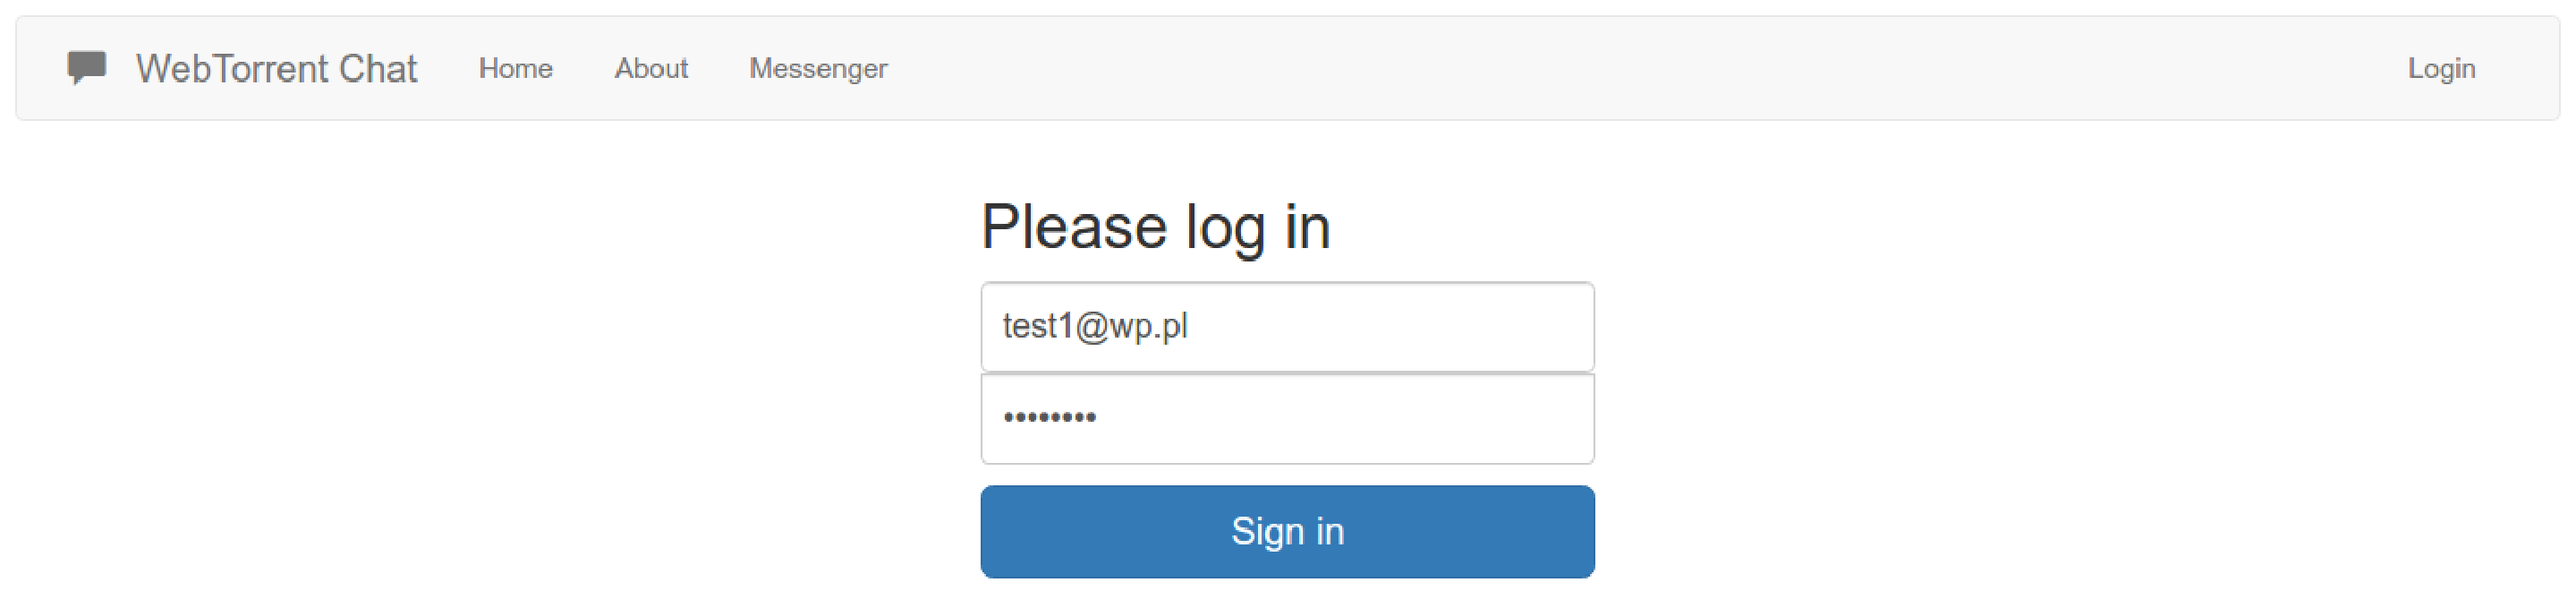
\includegraphics[width=1\linewidth]{img/logowanie}

\caption{Ekran logowania\label{fig:Ekran-logowania}}

\end{figure}

\subsection{Inicjalizacja modułów}

Poprawne zalogowanie do serwisu pozwala na przejście do głównego ekranu
komunikatora (przedstawiony na rysunku \ref{fig:Wygl=000105d-aplikacji-klienta}).
Po wyświetleniu tego widoku następuje pobranie z~serwera REST niezbędnych
informacji o~konwersacji (jeśli użytkownik już w~jakiejś uczestniczy),
uruchomienie modułu torrent (wykorzystującego bibliotekę WebTorrent,
odpowiedzialnego za wymianę wiadomości) oraz modułu, którego zadaniem
jest przechowywanie posiadanych wiadomości i~kontakt z~bazą danych
wbudowaną w~przeglądarkę. Szczegółowo ten proces został omówiony
poniżej.

Jeśli użytkownik był zapisany do konwersacji to klient pobiera z~serwera
REST szczegółowe informacje o~tej konwersacji (atrybuty przedstawione
w~punkcie \ref{subsec:Konwersacje}) oraz dane o~innych uczestnikach
tej konwersacji — między innymi ich identyfikator user\_dht\_id, który
jest niezbędny w~procesie odbierania wiadomości. Jeżeli użytkownik
nie uczestniczył jeszcze w~żadnej konwersacji to wyświetlone zostaje
pole umożliwiające podanie jej nazwy (conversation\_id) — rysunek
\ref{fig:Do=000142=000105czanie-do-konwersacji}. Szczegóły dołączania
do konwersacji opisano w~punkcie \ref{subsec:utw-dolacz-do-konwersacji}.

Kolejnym krokiem jest uruchomienie modułu odpowiedzialnego za przechowywanie
wiadomości (nazywany dalej modułem wiadomości). Moduł korzysta z~bazy
danych typu klucz-wartość znajdującej się w~przeglądarce (IndexedDB)
do \glqq trwałego'' zapisywania wysłanych i~odebranych wiadomości.
Słowo \glqq trwałego'' jest ujęte w~cudzysłów, ponieważ użytkownik
może w~każdej chwili usunąć dane. Jedynym sposobem, by je w~takiej
sytuacji odzyskać jest pobranie ich od innego użytkownika. Podczas
inicjalizacji moduł wczytuje do pamięci podręcznej wszystkie wiadomości
znajdujące się w~bazie danych — dzięki temu będą one dostępne dla
modułu torrent.

Ostatni etap przygotowania aplikacji do pełnego działania wymaga uruchomienia
modułu torrent obsługującego komunikację poprzez protokół BitTorrent.
W~ramach inicjalizacji moduł włącza klienta sieci P2P i~rozpoczyna
ponowne udostępnianie posiadanych wiadomości.

\subsection{Utworzenie lub dołączenie do konwersacji }

\label{subsec:utw-dolacz-do-konwersacji}

W celu prowadzenia rozmowy z~użytkownikami konieczne jest dołączenie
do wspólnej konwersacji. Rysunek \ref{fig:Do=000142=000105czanie-do-konwersacji}
pokazuje formularz umożliwiający utworzenie nowej rozmowy lub podanie
nazwy istniejącej. Użytkownik może rozpocząć nową konwersację i~poczekać,
aż inni do niej dołączą lub samemu dołączyć do już istniejącej. 

\begin{figure}[tbph]
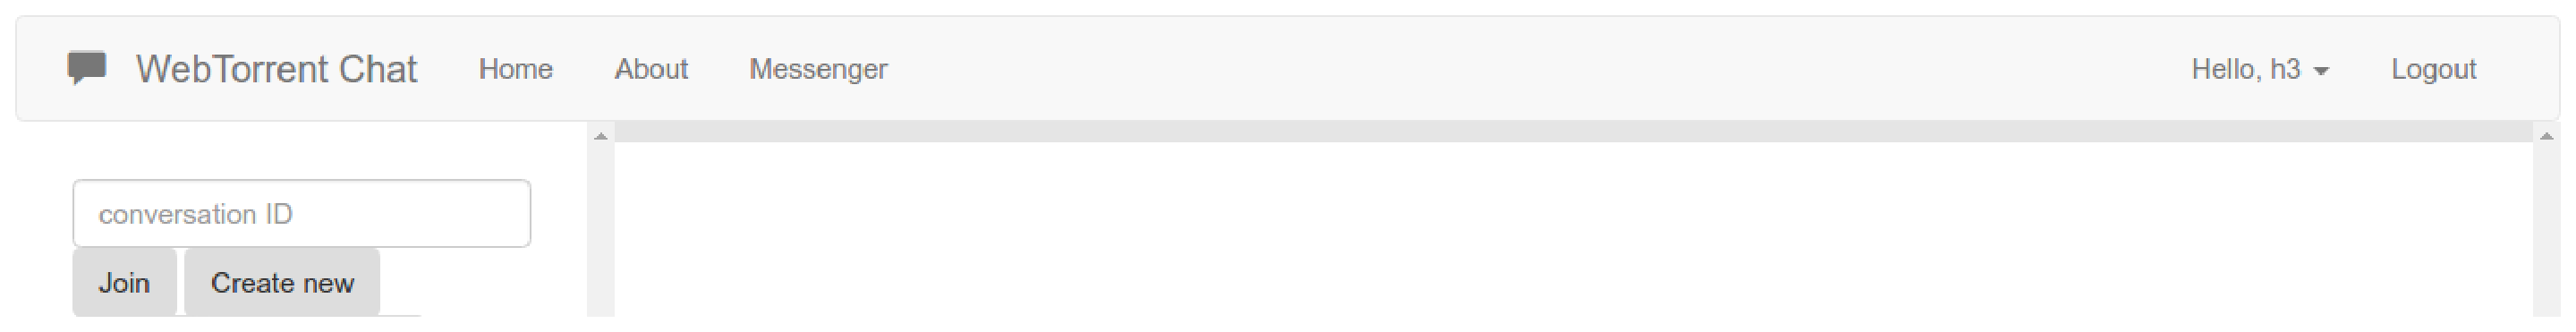
\includegraphics[width=1\linewidth]{img/dolacz}

\caption{Dołączanie do konwersacji\label{fig:Do=000142=000105czanie-do-konwersacji}}
\end{figure}

W pierwszym przypadku użytkownik wybiera opcję \glqq Create new''.
Aplikacja wysyła do serwera REST żądanie stworzenia konwersacji o~losowej
nazwie. Serwer automatycznie dołącza użytkownika do nowej konwersacji
i~odpowiada odsyłając nazwę konwersacji (conversation\_id). Użytkownik
zobaczy tę nazwę w~polu \glqq conversation ID''. Zadaniem użytkownika
jest teraz rozesłanie nazwy konwersacji do osób, z~którymi chce prowadzić
rozmowę. Może to zrobić, podobnie jak w~przypadku komunikatora Darkwire
(\ref{sec:Darkwire}), na przykład za pośrednictwem e-mail, SMS lub
przekazać osobiście.

Drugi przypadek zakłada, że użytkownik otrzymał od kogoś nazwę konwersacji
— wpisuje ją w~pole \glqq conversation ID'' i~zatwierdza przyciskiem
\glqq Join''. Klient wysyła do serwera REST żądanie, a~serwer zapisuje
w~bazie danych fakt dołączenia użytkownika do konwersacji. Serwer
w~odpowiedzi informuje klienta o~pomyślnym zakończeniu procedury. 

Dodatkowym założeniem, które należy spełnić w~obu przypadkach przed
dołączeniem do konwersacji jest posiadanie przez użytkownika unikalnego
user\_dht\_id (atrybut z~punktu \ref{subsec:Konwersacje}). Jest
to klucz w~DHT, pod którym użytkownik umieszcza informację o~najnowszej
wysłanej przez siebie wiadomości (jej info hash). Wartość user\_dht\_id
powinna być unikalna. Należy ją przesłać razem z~żądaniem opisanym
w~powyższych przypadkach. 

\subsection{Struktura komunikatu}

\label{subsec:Struktura komunikatu}

Wiadomość przesyłana między uczestnikami rozmowy ma następującą strukturę:
\begin{itemize}
\item content (treść wiadomości),
\item type (typ wiadomości, tekst, plik lub kontrolna),
\item timestamp (znacznik czasu nadania wiadomości),
\item sender (nadawca wiadomości),
\item previousInfoHash (wartość info hash poprzedniej wiadomości).
\end{itemize}
Z własności protokołu BitTorrent wynika, że torrenty są niezmienne
(ang. \dcsemph{immutable}) — zawartość plików lub ich liczba nie
może ulec zmianie bez zmiany wartości info hash. Konieczne zatem było
przyjęcie założenia, że każda nowa wiadomość wysłana przez użytkownika
staje się nowym torrentem. Scenariusz, w~którym użytkownik dodaje
wiadomość jako kolejny plik do istniejącego torrenta jest na chwilę
obecną niemożliwy do zrealizowania, chociaż istnieją próby wdrożenia
takiej możliwości (w~protokole BitTorrent \cite{bep39-bt,bep46-bt}
oraz w~bibliotece WebTorrent \cite{bep46-wt}). Niemniej jednak,
zdecydowano o~zachowaniu przyjętego założenia. 

Zastosowanie znaczników czasowych pozwala na zdefiniowanie kolejności
wiadomości — ich odbiorcy będą w~stanie posortować odbierane komunikaty
zgodnie z~porządkiem FIFO. Znaczniki dodatkowo gwarantują globalne
uporządkowanie wiadomości (ang. \dcsemph{total order}) — jeśli wszyscy
użytkownicy uczestniczący w~jednej konwersacji odbiorą wszystkie
wiadomości (każdy będzie posiadał identyczny zbiór), to zobaczą je
w~takiej samej kolejności. W~trakcie implementowania projektu zdecydowano,
że każda odebrana wiadomość będzie natychmiast wyświetlana — aplikacja
nie czeka na pobranie starszych wiadomości wysłanych przez danego
nadawcę. Narusza to co prawda oba wspomniane założenia, ale jedynie
tymczasowo, do momentu pobrania wszystkich wcześniejszych wiadomości.
Od tej chwili założenia pozostają spełnione. 

Użycie znaczników nie gwarantuje jednak przyczynowego uporządkowania
(ang. \dcsemph{causal order}), ponieważ zegary na maszynach użytkowników
nie są zsynchronizowane. W~większości przypadków \dcsemph{niewielka}
różnica czasu pozwoli na zachowanie uporządkowania przyczynowego.
\dcsemph{Niewielka} różnica czasu $\Delta t$ pomiędzy zegarami na
maszynach dwóch użytkowników $U_{N}$ (użytkownik-nadawca) i~$U_{O}$
(użytkownik-odbiorca) oznacza, że $\Delta t<min(t)+t_{0}$, gdzie:
\begin{itemize}
\item $min(t)$ to minimalny czas, który upłynie od momentu nadania wiadomości
$m$ przez $U_{N}$ (ustawienia czasu nadania w~polu timestamp) do
momentu odebrania wiadomości $m$ przez $U_{O}$ (wyświetlenia wiadomości
$m$ u~odbiorcy), 
\item $t_{0}$ to czas potrzebny na napisanie i~nadanie odpowiedzi zależnej
przyczynowo od wiadomości $m$ przez $U_{O}$, przy czym w~ogólności
może on wynosić 0 (zero).
\end{itemize}
Możliwy jest jednak następujący scenariusz:
\begin{enumerate}
\item $\Delta t>min(t)$, $t_{0}=0$.
\item $T_{N}>T_{O}$, gdzie $T_{N}$ i~$T_{O}$ to stan zegara maszyny
nadawcy/odbiorcy w~danym momencie, a~nierówność oznacza, że gdyby
porównać w~tym samym momencie zegary obu maszyn, to zegar maszyny
nadawcy będzie wskazywał wyższą wartość.
\item $U_{N}$ wysyła wiadomość $m$.
\item $U_{O}$ odbiera wiadomość $m$ i~od razu na nią odpowiada ($t_{0}=0$),
wysyłając wiadomość $n$. Timestamp ustawiony w~odpowiedzi $n$ będzie
miał niższą wartość niż timestamp otrzymany w~wiadomości $m$. Zarówno
$U_{N}$ jak i~$U_{O}$ zaobserwują ten fakt — wiadomość $n$ zostanie
wyświetlona powyżej wiadomości $m$ (co oznacza, że została wysłana
wcześniej). 
\end{enumerate}

\subsection{Wysłanie wiadomości i~algorytm ZLT}

\label{subsec:Wysy=000142anie wiadomo=00015Bci}

Aby wysłać wiadomość użytkownik podaje jej treść w~polu \glqq Type
message'' i~zatwierdza przyciskiem \glqq Send''. Dalsze czynności
wykonuje moduł torrent. Najpierw tworzy strukturę wiadomości (szerzej
opisaną w~punkcie \ref{subsec:Struktura komunikatu}). Następnie
rozpoczyna udostępnianie komunikatu w~sieci P2P zgodnie z~opisem
z~punktu \ref{subsec:Scenariusz utworzenia torrenta} (jest to zadanie
biblioteki WebTorrent). Kolejnym krokiem jest zapamiętanie info hasha
udostępnionej wiadomości. Klient zapisuje komunikat za pośrednictwem
modułu wiadomości w~bazie danych IndexedDB — kluczem jest info hash,
a~wartością struktura wiadomości. 

W trakcie implementowania programu zaobserwowano, że wraz ze wzrostem
liczby wiadomości umieszczanie każdej z~nich w~osobnym torrencie
bardzo szybko prowadzi do nadmiernego zużywania zasobów, a~nawet
do błędnego zakończenia programu. Z~tego powodu zdecydowano o~zaprojektowaniu
i~wdrożeniu algorytmu zmniejszającego liczbę jednocześnie udostępnianych
torrentów (nazywany dalej \dcsstrong{algorytmem ZLT} — Zmniejszającym
Liczbę Torrentów). Polega on na okresowym zastępowaniu torrentów zawierających
pojedynczą wiadomość (poziom 0) jednym torrentem (nazywanym dalej
\dcsstrong{torrentem kontrolnym}), który składa się z~wielu wiadomości
(poziom 1). Algorytm wykonuje się rekurencyjnie — jeśli powstanie
zbyt dużo torrentów kontrolnych na poziomie 1 to zostaną one połączone
w~jeden torrent kontrolny na poziomie 2, itd. Algorytm uruchamiany
jest jako kolejny krok po zleceniu zapisu do bazy danych. Został opisany
szczegółowo poniżej:
\begin{enumerate}
\item Jeżeli na danym poziomie znajduje się zbyt dużo wiadomości (więcej
niż zadany próg) to rozpocznij procedurę zamieniania wielu torrentów
w~jeden torrent kontrolny. W~przeciwnym przypadku zakończ algorytm.
\item Stwórz listę wiadomości, które znajdą się w~nowym torrencie kontrolnym.
\item Stwórz listę info hashy, które posiadają wiadomości znajdujące się
na liście w~punkcie 2. Dodatkowo, jeśli torrent kontrolny będzie
zastępował inne torrenty kontrolne, stwórz listę info hashy zastępowanych
torrentów kontrolnych.
\item Stwórz strukturę wiadomości (punkt \ref{subsec:Struktura komunikatu}),
w~polu \glqq treść'' umieść listy z~punktu 3.
\item Usuń z~klienta sieci P2P torrenty o~info hashach znajdujących się
na listach z~punktu 3. Usunięcie wykonywane jest z~opóźnieniem (domyślnie
po 5~sekundach).
\item Rozpocznij udostępnianie pliku składającego się z~wszystkich wiadomości
z~punktu 2 oraz wiadomości z~punktu 4 — procedura identyczna jak
wysyłanie zwykłej wiadomości. W~bazie danych zapisywana jest wiadomość
z~punktu 4 oraz usuwane z~niej są te zastąpione. 
\item Jeśli stworzenie nowego torrenta kontrolnego spowodowało, że na jego
poziomie znalazło się zbyt wiele torrentów, wykonaj algorytm dla tego
poziomu (od punktu 1).
\end{enumerate}
Po zakończeniu algorytmu należy wykonać ostatni krok, którym jest
umieszczenie wartości najnowszego info hasha w~DHT pod kluczem user\_dht\_id.
Działanie DHT zostało szczegółowo opisane w~punkcie \ref{sec:DHT}. 

Dla poprawnego działania programu kluczowe jest, by procedura wysyłania
kolejnej wiadomości $m_{j}$ rozpoczęła się dopiero po zakończeniu
procedury dla poprzedniej wiadomości $m_{i}$. Wynika to z~konieczności
podania wartości info hash wiadomości $m_{i}$ w~strukturze wiadomości
$m_{j}.$

Domyślnie algorytm umieszcza 5 wiadomości w~torrencie kontrolnym.
W~teście przedstawionym w~punkcie \ref{sec:wp=000142yw liczby wiad w zlt}
zbadano działanie aplikacji, gdy ta liczba jest inna.

Zaletą algorytmu ZLT jest znaczne zmniejszenie liczby jednocześnie
udostępnianych torrentów, a~to obniża zużycie zasobów. Wadą natomiast
jest powtórne wysyłanie wiadomości, które uczestnicy rozmowy mogli
już wcześniej odebrać — przykładowo, klient odebrał 4 kolejne wiadomości
będące pojedynczymi torrentami, a~następnie pobrał torrent kontrolny
zawierający 5 wiadomości, spośród których 4 już posiada i~jedną nową.
Oznacza to, że 80\% przesłanych danych było zbędne. 

\subsection{Odebranie wiadomości}

\label{subsec:Odebranie_wiadomo=00015Bci}

Procedura odebrania wiadomości rozpoczyna się okresowym sprawdzeniem
najnowszej wartości info hash w~DHT dla kluczy user\_dht\_id poszczególnych
uczestników rozmowy. Moduł torrent sprawdza, czy torrenty o~tych
info hashach znajdują się na liście pobieranych torrentów lub czy
zostały już pobrane i~znajdują się na liście wiadomości w~module
wiadomości. Jeśli żaden z~powyższych warunków nie jest spełniony,
wtedy na podstawie wartości info hash tworzony jest magnet link i~rozpoczyna
się procedura pobrania torrenta (punkt \ref{subsec:Scenariusz pobrania torrenta}).
Biblioteka WebTorrent pozwala na zarządzanie plikami w~trakcie ich
pobierania — możliwe jest odczytanie zawartości wiadomości pobranych
w~całości, podczas gdy pozostałe pliki są dalej przesyłane. Odczytana
wiadomość zostaje zapisana za pośrednictwem modułu wiadomości w~bazie
danych IndexedDB oraz na liście wiadomości do wyświetlenia użytkownikowi.
Oprócz tego moduł torrent sprawdza, czy poprzednia wiadomość wysłana
przez nadawcę znajduje się na liście wiadomości lub liście pobieranych
torrentów. Jeśli nie — moduł rozpoczyna procedurę pobierania tej wiadomości.

W sytuacji, gdy pobrano torrent kontrolny, moduł torrent usuwa z~klienta
sieci P2P torrenty, które znajdują się na liście przesłanej w~polu
\glqq treść'' wiadomości. Moduł zapisuje również w~bazie danych
brakujące wiadomości, o~ile istnieje taka konieczność. Podobnie jak
w~przypadku zwykłego torrenta, jeśli brakuje poprzedniej wiadomości,
moduł zacznie jej pobieranie. 

Koncepcja wysyłania i~odbierania wiadomości wykorzystująca protokół
BitTorrent umożliwia odebranie wiadomości nawet w~sytuacji, gdy jej
nadawca nie jest dostępny. Warunkiem koniecznym jest oczywiście dostępność
innego uczestnika rozmowy, który zdążył tę wiadomość pobrać, lub obecność
wielu użytkowników, z~których każdy posiada fragmenty wiadomości
(ang. \dcsemph{pieces}). W~drugim przypadku niezbędne jest założenie,
że każdy fragment (ang. \dcsemph{piece}) torrenta został pobrany
przez co najmniej jednego użytkownika.

\subsection{Udostępnianie starych torrentów}

\label{subsec:Udost=000119pnianie starych torr}

W celu zmniejszenia liczby torrentów, które klient w~danej chwili
pobiera i~wysyła, zdecydowano o~wprowadzeniu mechanizmu ograniczającego
udostępnianie starych wiadomości. Przyjęto założenie, że każdy uczestnik
rozmowy będzie pobierał wszystkie nowe wiadomości minimum raz w~tygodniu.
Podczas inicjalizacji modułu torrent każdy klient rozpoczyna ponowne
udostępnianie jedynie tych wiadomości i~torrentów kontrolnych, których
data wysłania jest młodsza niż 1 tydzień. Możliwy jest przypadek,
w~którym udostępniany torrent kontrolny zawiera wiadomości starsze
niż 1 tydzień — przyjęto, iż jest to sytuacja zgodna z~oczekiwaniami.
Wiadomości te i~tak przestaną być udostępniane maksymalnie w~ciągu
tygodnia ze względu na przedawnienie torrenta kontrolnego, który je
zawiera.

Wadą tego rozwiązania jest brak możliwości przeczytania wiadomości
starszych niż 1 tydzień przez osoby, które dopiero dołączyły do rozmowy.
Zdecydowano, że nie jest to poważny błąd, a~wręcz zaleta w~sytuacji,
gdy konwersacja zawiera dużą liczbę wiadomości. Dołączający klient
zmuszony byłby do pobrania całej historii konwersacji, co może być
operacją kosztowną komunikacyjnie.

\subsection{Zbiór sąsiadów}

W~ramach pojedynczej konwersacji klienty wysyłają i~odbierają wiadomości.
Każda wiadomość zostaje umieszczona w~osobnym torrencie, a~te mogą
zostać połączone w~nowy torrent kontrolny przez algorytm ZLT. Wszelka
wymiana danych pomiędzy klientami odbywa się zatem w~swarmach, dla
każdego torrenta z~osobna. Struktura (np. łańcuch, pierścień czy
graf pełny) jaką utworzą peery w~swarmie zależy od postępu algorytmu
wymiany danych. Możliwe jest ręczne zarządzanie listą peerów, z~którymi
dany klient posiada nawiązane połączenia, jednak w~ramach systemu
komunikatora nie zdecydowano się na ten krok — rolę zarządcy wystarczająco
dobrze spełniają algorytmy wbudowane w~protokół BitTorrent. W~trakcie
działania aplikacji i~tworzenia przez użytkowników nowych wiadomości,
klienty dynamicznie dołączają do powstających swarmów oraz odłączają
się od tych, które przestały funkcjonować, gdyż dany torrent został
zastąpiony przez nowy (kontrolny). 

Konwersacje są odseparowane od siebie, co oznacza, że klienty nie
nawiązują połączeń z~peerami znajdującymi się w~swarmach należących
do innej rozmowy. 

\section{DHT}

\label{sec:DHT}

Moduł DHT, czyli rozproszona tablica mieszająca, jest systemem składającym
się z~wielu węzłów pozwalającym na przechowywanie informacji. Węzłem
staje się każdy klient systemu komunikatora. Węzły dzielą między sobą
pewien zbiór kluczy i~posiadają możliwość komunikowania się z~innymi
węzłami i~przesyłania im posiadanych informacji. Zadaniem węzła jest
przechowywanie informacji dotyczących przypisanego mu podzbioru kluczy.
Każda informacja zapisywana w~DHT posiada etykietę (w~przypadku
systemu komunikatora jest nią user\_dht\_id), która następnie zamieniana
jest na klucz przez funkcję haszującą. Informacją w~systemie komunikatora
jest info hash najnowszej wysłanej przez klienta wiadomości. 

Przed przystąpieniem do pracy nad projektem zakładano, że biblioteka
WebTorrent jest wyposażona w~mechanizm opisany powyżej. Jest to częściowo
prawda — wersja biblioteki dla programów na platformę Node.js posiada
taką możliwość. Niestety brakuje jej w~wersji dla przeglądarek. Powody
dla braku wsparcia DHT w~bibliotece WebTorrent w~przeglądarce są
następujące:
\begin{itemize}
\item Przeglądarki mogą komunikować się bezpośrednio ze sobą jedynie dzięki
protokołowi WebRTC. Funkcjonuje on poprawnie dla niewielkiej liczby
jednoczesnych połączeń, jednak na potrzeby zaimplementowania DHT konieczne
byłoby utrzymywanie większej liczby równoległych połączeń, co może
prowadzić do szybkiego wyczerpania zasobów przeglądarki.
\item Jednym ze sposobów zaimplementowania DHT dla biblioteki WebTorrent
jest zaadaptowanie algorytmu Kademlia działającego już dla protokołu
BitTorrent. Wymaga on jednak zapamiętywania listy węzłów, z~którymi
dany węzeł nawiązał dotychczas połączenie, a~to oznacza, że połączenia
WebRTC muszą pozostać otwarte (nie można ich zakończyć). Jest to o~wiele
bardziej kosztowne w~przypadku WebRTC niż w~oryginalnej implementacji,
która korzysta z~bezpołączeniowego protokołu komunikacji UDP.
\item Kolejnym, bardzo istotnym problemem jest brak wsparcia protokołu WebRTC
dla dedykowanych wątków roboczych (ang. \dcsemph{WebWorker}, \dcsemph{ServiceWorker},
itp.). Bez tego wsparcia kod obsługujący DHT musi być wykonywany w~głównym
wątku danej strony internetowej, a~to może doprowadzić nawet do całkowitego
zablokowania interfejsu. W~chwili obecnej trwają próby wprowadzenia
wsparcia protokołu dla wątków roboczych — być może w~przyszłości
ten problem zostanie rozwiązany. 
\end{itemize}
W zaistniałej sytuacji przeprowadzono poszukiwania alternatywnej biblioteki
udostępniającej mechanizm DHT dla przeglądarek. Znalezione biblioteki
pozwalały programiście na zdefiniowanie kanału wymiany informacji
pomiędzy węzłami \cite{kademlia-dht} lub posiadały działający mechanizm
\cite{kadtools}. Jednakże w~trakcie wstępnych testów okazało się,
że żadna biblioteka nie zapewnia satysfakcjonujących rezultatów —
informacje były przesyłane zbyt długo lub w~ogóle nie docierały do
niektórych węzłów. 

Ze względu na brak zaimplementowanego mechanizmu DHT w~bibliotece
WebTorrent oraz niesatysfakcjonujące alternatywy zdecydowano o~zastąpieniu
tego mechanizmu atrapą (mock). Funkcjonalność tego rozwiązania pozostaje
niezmienna — każdy klient ma możliwość zapisania najnowszej wartości
info hash pod określonym kluczem (user\_dht\_id) oraz odczytania tej
informacji. Zmianie uległ sposób przechowywania informacji — zadanie
to nie należy już do sieci powiązanych ze sobą klientów, a~stało
się jednym z~zadań serwera REST. Serwer udostępnia ścieżkę REST /dht,
która umożliwia następujące akcje:
\begin{itemize}
\item metoda HTTP GET z~parametrem user\_dht\_id pozwala na pobranie wartości
przechowywanej dla klucza user\_dht\_id,
\item metoda POST pozwala na zapisanie wartości dla klucza user\_dht\_id.
\end{itemize}

\section{Bezpieczeństwo i~kryptografia w~języku JavaScript}

\label{sec:Bezpiecze=000144stwo, krypto, JS}

Mobilne i~dektopowe klienty aplikacji Bleep (punkt \ref{sec:bleep})
oraz aplikacji Signal (punkt \ref{sec:signal}) oferują szyfrowanie
wiadomości. Webowy klient aplikacji Darkwire (punkt \ref{sec:Darkwire})
również. W~ramach niniejszej pracy magisterskiej zbadano sposób implementacji
tego mechanizmu w~przytoczonych aplikacjach oraz podjęto próbę zaprojektowania
go dla systemu komunikatora. 

Poufność wiadomości w~systemie komunikatora jest konieczna, ponieważ
każdy użytkownik systemu (ale też osoba spoza niego) ma możliwość
pobrania i~odczytania treści wiadomości przesyłanych jako torrenty.
Gdyby wiadomość była zaszyfrowana, posiadanie jej w~takiej formie
nie powoduje negatywnych skutków. Głównym problemem do rozwiązania
jest przechowywanie kluczy pozwalających na odczytanie zaszyfrowanych
wiadomości i~podpisywanie wysyłanych treści. Problem przechowywania
dotyczy zarówno zarządzania kluczami w~trakcie pracy aplikacji jak
i~po jej zamknięciu — zapisanie kluczy w~pamięci trwałej. Klucz
prywatny nie powinien być wysyłany poza urządzenie, na którym został
wygenerowany. 

Ostatecznie zrezygnowano z~wdrożenia szyfrowania wiadomości, choć
technicznie jest to osiągalne, ponieważ mechanizm ten posiadałby istotne
wady mogące powodować brak gwarancji poufności przesyłanych danych.
Podsumowanie badań opisano w~poniższych punktach.

\subsection{Darkwire}

\label{subsec:darkwire-bezpieczenstwo}

Aplikacja webowa Darkwire automatycznie szyfruje wiadomości w~przeglądarce
użytkownika przed wysłaniem ich do serwera. Serwer przesyła wiadomości
do odbiorców, a~po dotarciu do nich, treść jest odszyfrowywana. W~programie
zastosowano kryptografię klucza publicznego do stworzenia klucza symetrycznego
danej wiadomości. Aplikacja korzysta z~Web Cryptography API \cite{web cryptography api}
do zarządzania kluczami kryptograficznymi. 

Scenariusz uruchomienia programu i~przesłania zaszyfrowanej wiadomości
jest następujący \cite{darkwire szyfrowanie how it works}:
\begin{enumerate}
\item Podczas uruchomienia, program tworzy nową rozmowę (ang. \dcsemph{chat room})
oraz parę kluczy (publiczny i~prywatny). 
\item W momencie dołączenia nowej osoby do rozmowy, aplikacje użytkowników
wymieniają się kluczami publicznymi uczestników rozmowy. 
\item W celu wysłania wiadomości program najpierw generuje 3 nowe klucze:
symetryczny klucz sesji, klucz podpisujący (umożliwiający weryfikację
sygnatury wiadomości) oraz wektor inicjujący (ang. \dcsemph{initialization vector}). 
\item Treść wiadomości zostaje zaszyfrowana przy pomocy klucza sesji i~wektora
inicjującego. Oprócz tego tworzona jest sygnatura wiadomości przy
użyciu klucza podpisującego. 
\item Klucz sesji i~klucz podpisujący zostają zaszyfrowane kluczami publicznymi
odbiorców, dla każdego z~osobna — ta technika pozwala na uniknięcie
szyfrowania całej treści wiadomości osobno dla wszystkich odbiorców. 
\item Ostatnim krokiem przed wysłaniem wiadomości jest przygotowanie paczki
danych do wysłania — składa się ona z~zaszyfrowanej wiadomości, wektora
inicjującego, sygnatury wiadomości, zaszyfrowanego klucza sesji oraz
zaszyfrowanego klucza podpisującego. 
\item Odbiorca, po otrzymaniu takiej paczki danych, odszyfrowuje swoim kluczem
prywatnym klucze sesji oraz klucz podpisujący. Używając odszyfrowanego
klucza sesji i~wektora inicjującego odbiorca odszyfrowuje treść wiadomości
i~może zweryfikować sygnaturę wiadomości odszyfrowanym kluczem podpisującym. 
\end{enumerate}
Przedstawiony scenariusz gwarantuje poufność wiadomości i~autentyczność
odbiorcy podczas normalnej pracy aplikacji. Istnieją jednak wektory
ataku pozwalające na zdobycie kluczy prywatnych i~w~konsekwencji
na odczytanie przesłanych wiadomości czy przejęcie kontroli nad kontem
użytkownika i~podszywanie się pod nadawcę. Głównym problemem z~punktu
widzenia bezpieczeństwa jest przechowywanie klucza prywatnego jako
wartość zmiennej w~skrypcie JavaScript (lub w~niezabezpieczony sposób
w~local storage czy IndexedDB). Wykorzystując choćby atak XSS (ang.
\dcsemph{Cross-site scripting}), czyli uruchomienie własnego skryptu
osadzonego w~treści atakowanej strony, można pozyskać wrażliwe dane.
Zmiany w~kodzie strony może dokonać nie tylko cracker, ale również
twórca oprogramowania z~własnej woli lub zmuszony przez trzecią stronę
(np. agencję rządową). 

Użycie powyższej metody do przechowywania wrażliwych danych może prowadzić
do ich kradzieży i~ujawnienia treści wiadomości. Jako usprawiedliwienie
można podać przykład Messengera (punkt \ref{sec:messenger}), który
nie stosuje w~ogóle szyfrowania wiadomości — jedynym zabezpieczeniem
jest przesyłanie ich do serwera szyfrowanymi kanałami. W~bazie danych
są one zapisywane w~takiej samej formie, w~jakiej zostały wprowadzone
przez użytkownika. Zdobycie dostępu do bazy danych przez osoby niepowołane
spowoduje ujawnienie treści wiadomości. Niemniej jednak, taki wektor
ataku wydaje się być mniej prawdopodobny — bazy danych są zazwyczaj
lepiej zabezpieczone niż komputery użytkowników.

W aplikacjach webowych istnieje jeszcze inna możliwość przesyłania
i~przechowywania poufnych informacji (np. tokenów uwierzytelniających),
a~mianowicie ciasteczka (ang. \dcsemph{cookies}). Te małe fragmenty
tekstu są wysyłane przez serwer do klienta w~nagłówku HTTP, a~przeglądarka
odsyła je wraz z~kolejnymi żądaniami. W~celu zabezpieczenia tych
informacji stosuje się szyfrowany protokół (np. HTTPS) oraz ustawia
niezbędne flagi (jak choćby httpOnly, secure, domain, path itd.).
Ustawienie pierwszej flagi skutkuje brakiem dostępu do zawartości
ciasteczka z~poziomu kodu JavaScript. Niestety w~systemie komunikatora
ten sposób przechowywania poufnych informacji nie może być wykorzystany,
gdyż większość operacji wykonywanych jest z~poziomu skryptu, a~komunikaty
przesyłane są innymi protokołami niż HTTP. 

\subsection{Bleep i~Signal}

Natywne aplikacje mobilne mają nad aplikacjami webowymi istotną przewagę
— umożliwiają programistom dostęp do pamięci trwałej urządzenia. Dodatkowo,
systemy mobilne zwiększają bezpieczeństwo przechowywanych informacji
poprzez izolację danych zapisywanych przez konkretną aplikację — inne
programy nie mają dostępu do tych obszarów. Ta możliwość pozwala na
znacznie bezpieczniejsze przechowywanie poufnych danych. Wszelkie
operacje związane z~szyfrowaniem odbywają się na urządzeniach użytkowników.

Oprócz tego, twórcy przytoczonych aplikacji zastosowali znacznie bardziej
rozbudowany mechanizm przesyłania wiadomości niż w~przypadku aplikacji
Darkwire. W~aplikacji Signal wprowadzono choćby \glqq The Double
Ratchet Algorithm'' \cite{signal double ratchet} — algorytm gwarantujący
własność utajnienia przekazywania (ang. \dcsemph{forward secrecy}).
Każda wiadomość jest szyfrowana innym kluczem. Ponadto, nawet jeśli
cracker uzyskałby dostęp do pojedynczej wiadomości i~jej metadanych,
nie może na ich podstawie obliczyć wartości poprzednich ani przyszłych
kluczy. Podobny mechanizm oferuje aplikacja Bleep \cite{bleep forward secrecy}. 

Twórcy aplikacji Bleep umożliwiają użytkownikom wysyłanie wiadomości
pod nieobecność odbiorcy — zapisywana jest ona wtedy w~DHT. Węzłami
w~DHT są aplikacje użytkowników, więc dane przechowywane w~DHT również
muszą być zaszyfrowane \cite{bleep forward secrecy offline}. Algorytm
jest podobny do przedstawionego powyżej z~niewielką zmianą — nowy
klucz generowany jest nie dla każdej wiadomości, a~dla paczki wiadomości
nadanych podczas nieobecności odbiorcy. Gdy odbiorca staje się dostępny,
odczytuje wiadomości i~generuje nowy klucz. 

\subsection{Inne pomysły i~wnioski}

Badanie rozwiązań wdrożonych w~powyższych aplikacjach doprowadziło
do powstania innych koncepcji rozwoju systemu komunikatora prowadzących
do zabezpieczenia konwersacji między użytkownikami. Przedstawione
zostały poniżej.
\begin{itemize}
\item Przechowywanie kluczy publicznych i~prywatnych w~bazie danych z~dostępem
poprzez serwer REST. Klucze mogą być generowane przez serwer lub przez
klienta. Rozwiązanie nie jest poprawne jeśli zakłada się, że nikt
poza nadawcą i~odbiorcami nie ma prawa odczytać treści wiadomości.
Jeśli jednak założenie to zostanie złagodzone i~oprócz wspomnianych
osób dostęp do treści wiadomości będzie miał zaufany serwer, rozwiązanie
mogłoby zostać wprowadzone. W~tej sytuacji uzyskuje się poziom poufności
podobny do aplikacji Messenger (punkt \ref{sec:messenger}), w~przypadku
której wiadomości również mogą być odczytane z~bazy danych. 
\item Rozwinięciem poprzedniego rozwiązania byłoby wygenerowanie pary kluczy
po stronie klienta oraz dodatkowe zabezpieczenie ich w~taki sposób,
by jedynie użytkownik miał możliwość odczytania ich po podaniu hasła
dostępu. Następnie zaszyfrowane dane są wysyłane do serwera i~tam
przechowywane. Na żądanie klienta, na przykład podczas uruchamiania
aplikacji, dane są pobierane, użytkownik podaje hasło i~uzyskuje
lokalnie dostęp do poufnych informacji. Niestety, oba rozwiązania
są w~dalszym ciągu podatne na kradzież danych — odszyfrowane klucze
są przetwarzane przez skrypt i~mogą zostać przechwycone.
\item Ostatnim, póki co koncepcyjnym, pomysłem jest zastosowanie Web Cryptography
API \cite{webCrypto API w3,webCrypto-experimental }. Konieczne jest
jednak założenie, że nie będzie istniała możliwość odczytania czy
importu kluczy prywatnych z~poziomu kodu JavaScript. Wszelkie operacje
na poufnych danych (generowanie kluczy, szyfrowanie i~odszyfrowywanie
danych) powinny być wykonywane przez algorytmy zaimplementowane bezpośrednio
w~przeglądarce — dzięki temu unika się przechowywania kluczy prywatnych
w~zmiennych i~ich przetwarzania przez kod JavaScript, a~to z~kolei
uniemożliwia ich kradzież. Algorytmy dostępne byłyby przez API. 
\end{itemize}

\section{Wykorzystane technologie}

Podczas pracy nad projektem systemu komunikatora użyto wielu technologii,
zwykle standardowych i~popularnych dla danej platformy. Język programowania
wykorzystany do implementacji serwera REST to język Python. Aplikacja
kliencka powstała w~języku JavaScript. 

Klient jest aplikacją webową typu Single Page Application. Do zaimplementowania
tego typu programu wykorzystano framework AngularJS, który został
opisany w~punkcie \ref{subsec:AngularJS}. W~punkcie \ref{subsec:grunt bower yo}
przedstawiono system budujący Grunt, menedżer pakietów Bower i~generator
szkieletu projektu Yeoman, które są zwykle wykorzystywane wraz z~frameworkiem
AngularJS. Oprócz standardowych funkcji dostępnych we wspomnianym
frameworku oraz w~języku JavaScript, skorzystano z~funkcji znajdujących
się w~bibliotece Lodash (pkt. \ref{subsec:lodash}). W~celu udostępnienia
zbudowanego projektu przez serwer aplikacji, zastosowano platformę
Node.js oraz framework Express (pkt. \ref{subsec:node}).

Serwer REST został napisany przy wykorzystaniu frameworka Python Eve
(pkt. \ref{subsec:py eve}). Do wymiany informacji pomiędzy serwerem
REST a~aplikacjami klienckimi wykorzystano format danych JSON (ang.
\dcsemph{JavaScript Object Notation}). Serwer zapisuje dane w~bazie
danych MongoDB (pkt. \ref{subsec:mongo}). 

W celu przeprowadzenia testów wydajności systemu komunikatora skorzystano
z~frameworka testującego Protractor (pkt. \ref{subsec:protractor}).
Jego zastosowanie jest rekomendowane dla aplikacji webowych wykorzystujących
AngularJS. Zbadanie danych wysyłanych i~odbieranych przez maszyny
testowe umożliwił analizator protokołów sieciowych Wireshark \cite{wireshark}. 

Wdrożenie systemu komunikatora było możliwe dzięki zastosowaniu platformy
chmurowej Heroku (pkt. \ref{subsec:heroku}).

\subsection{AngularJS}

\label{subsec:AngularJS}

AngularJS \cite{angularjs} to projekt na licencji MIT, rozwijany
głównie przez firmę Google. Framework ten umożliwia tworzenie i~rozwój
aplikacji internetowych typu Single Page Application. Znacznym ułatwieniem
podczas projektowania i~testowania aplikacji jest zastosowanie w~AngularJS
wzorca projektowego MVC (ang. \dcsemph{Model-View-Controller}). Pozwala
on między innymi na rozdzielenie warstw modelu (danych), widoku (prezentacji)
i~kontrolera (logiki), co z~kolei przyczynia się do zwiększenia
uporządkowania projektu. 

Ponadto, użycie wzorca projektowego wstrzykiwania zależności (ang.
\dcsemph{dependency injection}) daje możliwość zastosowania po stronie
klienta serwisów typowych dla aplikacji serwerowych. Jest to istotna
cecha, ponieważ system komunikatora w~znacznym stopniu polega na
współpracy klientów (komunikacja P2P). Rola serwera powinna być w~projekcie
jak najmniejsza.

Jedną z~najważniejszych funkcji AngularJS, redukującą ilość napisanego
kodu, jest mechanizm dwukierunkowego wiązania danych (ang. \dcsemph{two-way data binding}).
Umożliwia on dynamiczną zmianę widoku na skutek modyfikacji danych
w~modelu. Wszelkie operacje na modelu przeprowadzane są w~kontrolerze.
Ponadto, zmiany widoku również mogą wpływać na model — dlatego wiązanie
nazwane jest dwukierunkowym. 

\subsection{Grunt, Bower, Yeoman}

\label{subsec:grunt bower yo}

Grunt \cite{grunt} jest narzędziem automatyzującym powtarzalne czynności
w~trakcie projektowania aplikacji webowej. Narzędzie pozwala między
innymi na przygotowanie ostatecznej wersji projektu, gotowej do wdrożenia
na serwerze. 

Kolejnym przydatnym narzędziem jest Bower \cite{bower}. Jest to menedżer
umożliwiający definiowanie, jakie pakiety (biblioteki, moduły itp.)
zostaną użyte w~roboczej i~docelowej wersji projektu. Bower automatycznie
wyszukuje i~instaluje określoną lub najnowszą wersję każdego uwzględnionego
pakietu oraz sprawdza zależności między pakietami.

Yeoman \cite{yeoman} to generator szkieletu projektu. Jest on używany
jednorazowo na początku pracy i~pozwala na stworzenie pierwszej wersji
działającego systemu — podstawowej struktury katalogów projektu oraz
niezbędnych plików. Dzięki temu programista może skupić się, w~kolejnych
krokach, jedynie na istotnych i~unikalnych funkcjach systemu. 

\subsection{Lodash}

\label{subsec:lodash}

Lodash \cite{lodash} jest biblioteką udostępnioną na licencji MIT
i~dostarczającą programiście metody rozszerzające język JavaScript.
Zastosowanie biblioteki w~projekcie pozwala na przyspieszenie implementacji
systemu poprzez skorzystanie z~gotowych fragmentów kodu. Do dyspozycji
są między innymi metody operujące na ciągach znaków, tablicach, obiektach
i~kolekcjach obiektów. W~ramach biblioteki dostępne są również bardziej
wydajne zamienniki funkcji obecnych w~standardzie języka JavaScript
— ich użycie pozwala na przyspieszenie działania projektowanej aplikacji. 

\subsection{Node.js, Express}

\label{subsec:node}

Środowisko uruchomieniowe Node.js \cite{node} służy do tworzenia
skalowalnych aplikacji internetowych w~języku JavaScript. W~szczególności,
umożliwia zaprojektowanie serwerów WWW. W~niniejszym projekcie serwer
Node.js (wraz z~modułem Express \cite{express}) posłużył do udostępniania
gotowego programu klienckiego — umożliwia przeglądarkom pobranie aplikacji
komunikatora. 

Framework oraz moduły, które można użyć wraz z~nim, są projektami
open-source.

Npm \cite{npm} jest domyślnym menedżerem pakietów dla platformy Node.js.

\subsection{Python Eve}

\label{subsec:py eve}

Do implementacji serwera REST w~systemie komunikatora wykorzystano
framework Python Eve \cite{python-eve}. Do głównych zalet tego narzędzia
należy zaliczyć jego prostotę oraz przyjęcie pewnych konwencji — dzięki
temu programista definiuje tylko niezbędne, unikalne dla danego programu
elementy. W~szczególności, rolą projektanta jest sprecyzowanie klas
— określenie ich nazw i~atrybutów. W~przypadku systemu komunikatora
są to klasy użytkownika (punkt \ref{subsec:uzytkownicy i logowanie})
i~konwersacji (punkt \ref{subsec:Konwersacje}). Dodatkowo, należy
zdefiniować zależności pomiędzy klasami, ograniczenia integralnościowe
dla poszczególnych atrybutów oraz podstawową konfigurację połączenia
z~bazą danych. Wiele zadań, które powtarzają się w~projektach typowych
serwerów REST, jest zapewnionych automatycznie przez framework — są
to przykładowo: walidacja danych, przygotowanie ścieżek dostępu do
obiektów poprzez protokół HTTP czy obsługa bazy danych. Wybór tej
technologii wynika z~faktu, iż serwer w~systemie komunikatora pełni
jedynie rolę typowego pośrednika aplikacji klienckich z~bazą danych
i~nie wykonuje niestandardowych obliczeń (nietypowych dla serwera
REST). Możliwości oferowane przez framework Python Eve okazały się
wystarczające. System polega w~większości na współpracy aplikacji
klienckich. 

\subsection{MongoDB}

\label{subsec:mongo}

MongoDB \cite{mongo} jest systemem do zarządzania nierelacyjną bazą
danych. Zastosowanie tej bazy danych w~systemie komunikatora wynika
wprost z~faktu użycia frameworka Python Eve, który jest domyślnie
przystosowany do współpracy z~bazą danych MongoDB. Dane przechowywane
są w~niej w~formie dokumentów JSON. Baza danych charakteryzuje się
wysoką wydajnością i~skalowalnością. Ponadto, jest to oprogramowanie
open-source. 

W celu uruchomienia publicznie dostępnej bazy danych skorzystano z~mLab
\cite{mlab}. Jest to chmurowa platforma udostępniająca bazę danych
jako serwis (ang. \dcsemph{DaaS, Database as a~Service}). 

\subsection{Protractor}

\label{subsec:protractor}

Zalecanym frameworkiem testującym dla aplikacji napisanych przy użyciu
AngularJS jest Protractor \cite{protractor}. Pozwala on na zdefiniowanie
scenariuszy testowych oraz automatycznie przeprowadzenie zaplanowanych
testów. Możliwe jest również ustalanie parametrów testowych oraz warunków,
w~jakich poszczególne testy należy uznać za zakończone pomyślnie.
Zastosowanie tej technologii umożliwiło zbadanie wydajności systemu
komunikatora w~powtarzalny sposób. 

\subsection{Heroku }

\label{subsec:heroku}

Heroku \cite{heroku} to platforma chmurowa, działająca w~modelu
PaaS (ang. \dcsemph{Platform as a~Service}). Serwer REST oraz serwer
aplikacji zostały umieszczone w~wirtualnych środowiskach oferowanych
przez tę usługę. Dzięki temu obie aplikacje są dostępne publicznie
— posiadają publiczny adres IP oraz domenę internetową. Aplikacja
kliencka może komunikować się z~serwerem REST. Platforma Heroku umożliwia
między innymi zarządzanie aplikacjami, wyłączanie ich, modyfikację
ustawień oraz automatycznie buduje i~uruchamia nową wersję oprogramowania
po zaktualizowaniu jej kodu źródłowego w~publicznym repozytorium
kodu. 

\section{Dalszy rozwój}

\label{sec:Dalszy rozw=0000F3j}

Poniżej opisano pokrótce kilka idei rozwijających system komunikatora.

\subsection{Relacja znajomości}

Zaimplementowanie relacji znajomości pomiędzy użytkownikami. Dzięki
temu osoba tworząca konwersację będzie mogła od razu dopisać do niej
uczestników wybierając ich z~listy swoich znajomych. Kwestią do rozstrzygnięcia
pozostaje w~tej sytuacji wybranie, kto ma przypisać uczestnikom wartość
user\_dht\_id (osoba tworząca konwersację czy każdy jej członek z~osobna).

\subsection{Spójność przyczynowa}

Zagwarantowanie spójności przyczynowej wiadomości i~wyświetlanie
komunikatów dopiero, gdy pobrane zostały wszystkie poprzednie. Obie
własności spowodują bardziej realistyczne wrażenie prowadzenia rozmowy.
Jeśli użytkownik wysłał wiadomość \dcsemph{b} w~odpowiedzi na otrzymaną
wiadomość a~to pojawią się one w~oknie rozmowy w~odpowiedniej kolejności
— najpierw \dcsemph{a}, potem \dcsemph{b}. Jest to możliwe do osiągnięcia,
jeśli wiadomości będą zawierały zegar wektorowy z~wartościami ostatnio
odebranych wiadomości.

\subsection{Szyfrowanie wiadomości}

Sposoby implementacji oraz ich znane wady opisano w~punkcie \ref{sec:Bezpiecze=000144stwo, krypto, JS}.
Niemniej jednak ta własność jest niezbędna, by treść wiadomości nie
mogła zostać odczytana przez osoby niepowołane (użytkowników nie należących
do danej konwersacji). 

\subsection{Dostarczanie wiadomości}

\label{subsec:dostarczanie wiadomo=00015Bci offline propozycja}

Zagwarantowanie dostarczenia wiadomości w~sytuacji, gdy użytkownik
uruchamia aplikację i~żaden z~uczestników konwersacji nie jest dostępny.
Problem ten może zostać rozwiązany na przykład poprzez dodanie do
konwersacji serwera jako uczestnika. Serwer ten wykonywałby taki sam
kod programu jak inni klienci, ale nie miałby możliwości odszyfrowywania
wiadomości ani nadawania własnych komunikatów. Alternatywnym sposobem
rozwiązania problemu byłoby powierzenie przekazywania wiadomości programom
należącym do znajomych użytkowników. Oni również nie mieliby możliwości
odczytania i~modyfikacji treści wiadomości. 

\subsection{Lista info hashy zamiast pojedynczych wartości}

\label{subsec:lista IH zamiast pojedynczych warto=00015Bci}

Przechowywanie listy ostatnich wartości info hash w~DHT (zamiast
pojedynczej wartości) oraz przesyłanie jej w~strukturze wiadomości
(również zamiast pojedynczej wartości previousInfoHash). Dzięki temu
możliwe byłoby równoległe pobieranie wiadomości przez dołączających
klientów. Ponadto, to rozwiązanie pozwala na zmniejszenie skali problemu
nadpisywania wartości w~DHT — jeśli użytkownik wysyła wiadomości
w~szybkim tempie, to możliwe jest nadpisanie wartości info hash w~DHT,
zanim ktokolwiek zdąży ją odczytać.

\subsection{Zmiana zawartości torrenta bez zmiany info hasha}

\label{subsec:zmiana zawarto=00015Bci bez zmiany IH}

Modyfikacja protokołu BitTorrent pozwalająca na ponowne wykorzystanie
istniejących swarmów, ponieważ konieczność dołączania do nowego swarmu
dla każdej wysłanej wiadomości powoduje duży narzut komunikacyjny
wynikający z~nawiązywania połączenia pomiędzy peerami. Z~dużym prawdopodobieństwem
w~nowych swarmach znajdą się te same peery, które uczestniczyły w~udostępnianiu
poprzednich wiadomości. Alternatywnym sposobem rozwiązania tego problemu
jest możliwość dodawania nowych plików do istniejącego torrenta bez
zmiany wartości info hash — istnieją propozycje wprowadzenia takiej
modyfikacji protokołu \cite{bep39-bt,bep46-bt}. Klient dołącza wtedy
do tylu swarmów, ilu jest uczestników rozmowy i~nie opuszcza ich
aż do momentu, w~którym użytkownik zdecyduje o~wyłączeniu aplikacji.
Każda wiadomość byłaby wtedy nowym plikiem w~tym samym, istniejącym
już torrencie. Zaletą wynikającą z~omówionej modyfikacji jest znaczne
zmniejszenie liczby swarmów, w~których klient musi się jednocześnie
znajdować. Dodatkowo, w~drugim rozwiązaniu możliwe byłoby zrezygnowanie
z~algorytmu ZLT oraz wyeliminowanie ponownego wysyłania tych samych
wiadomości w~torrentach kontrolnych.

\subsection{Wysyłanie plików (zdjęć, filmów)}

Komunikatory wymienione w~rozdziale \ref{chap:istniejace rozwiazania}
posiadają możliwość wysyłania różnych plików jako załączniki lub jako
osobne wiadomości. Ponadto, częstą praktyką w~popularnych komunikatorach
jest umieszczanie w~aplikacji wbudowanych obrazów wyrażających określone
emocje, które użytkownik może przeszukiwać i~wysyłać. 

\chapter{Wyniki testów}

\label{chap:Wyniki test=0000F3w}

Po zakończeniu prac nad systemem komunikatora przeprowadzono serię
testów mających na celu zbadanie wydajności aplikacji. W~punkcie
\ref{sec:Kryteria} przedstawiono parametry, w~przypadku których
zmiana wartości mogłaby wpłynąć na wydajność aplikacji. W~punkcie
\ref{sec:Scenariusze testowe} przybliżono scenariusze testowe, a~w~punkcie
\ref{sec:specyfikacja} opisano specyfikację maszyn testowych. W~dalszej
części znajdują się szczegółowe opisy poszczególnych testów oraz wnioski,
które z~nich wynikają.

\section{Kryteria }

\label{sec:Kryteria}

Wymienione poniżej parametry umożliwiają symulację różnych sytuacji
podczas testów. Zmiana ich wartości może pozytywnie lub negatywnie
wpływać na wydajność aplikacji. Pod uwagę wzięto następujące kryteria:
\begin{enumerate}
\item rozmiar wiadomości,
\item liczba uruchomionych klientów (dostępnych użytkowników) oraz liczba
klientów wysyłających wiadomości,
\item liczba wiadomości w~konwersacji,
\item liczba wiadomości, która zostaje umieszczona w~torrencie kontrolnym,
\item sposób podłączenia klientów do sieci — czy klienty znajdują się w~jednej
lub różnych podsieciach oraz czy jest to sieć domowa, czy laboratoryjna,
\item zbadanie, czy uruchomienie w~jednej sieci wielu klientów obsługujących
różne konwersacje wpływa na wydajność. 
\end{enumerate}

\section{Scenariusze testowe}

\label{sec:Scenariusze testowe}

Zaproponowano następujące scenariusze:
\begin{enumerate}
\item Jeden nadawca wysyła wszystkie wiadomości bez czekania na odpowiedzi
— zmierzono czas otrzymania przez wszystkich odbiorców pełnej listy
wiadomości. 
\item Jeden nadawca $U_{N}$ wysyła wiadomość \dcsemph{m} i~czeka na odpowiedzi
od wszystkich odbiorców. Odpowiedzi są wysyłane natychmiast po otrzymaniu
wiadomości \dcsemph{m}. Zmierzono czas otrzymania poszczególnych
odpowiedzi przez nadawcę $U_{N}$ od momentu nadania wiadomości \dcsemph{m}.
Scenariusz ma symulować naturalną rozmowę, w~której uczestnicy odpowiadają
na otrzymaną wiadomość dopiero, gdy ją otrzymają. Pomiar czasu zaczyna
się w~momencie wysłania wiadomości przez nadawcę $U_{N}$, a~kończy
się w~momencie otrzymania przez nadawcę $U_{N}$ odpowiedzi od danego
odbiorcy (dla każdego odbiorcy z~osobna). Czas przesłania wiadomości
w~jedną stronę jest (uśredniając) połową uzyskanego wyniku. Nadawca
$U_{N}$ wyśle kolejną wiadomość dopiero po otrzymaniu wszystkich
odpowiedzi. 
\item Jeden klient dołącza do konwersacji. Zmierzono czas otrzymania pełnej
listy wiadomości przez dołączającego klienta.
\end{enumerate}

\section{Specyfikacja komputerów i~środowiska testowe}

\label{sec:specyfikacja}

Część testów przeprowadzono w~laboratorium wyposażonym w~komputery
stacjonarne posiadające adresy IP w~tej samej podsieci — komputer
tego typu będzie dalej oznaczony jako K1. Dodatkowo, w~powyższych
testach wykorzystano komputer podłączony do odrębnej podsieci (nazwany
dalej K2). Druga część testów została przeprowadzona na komputerach
podłączonych do jednej sieci domowej — w~tych testach wykorzystano
komputer K3 oraz komputer K4. Podział testów na części przeprowadzane
w~różnych środowiskach pozwolił na zwiększenie różnorodności konfiguracji
oraz zaobserwowanie zjawisk, które występują w~jednym ze środowisk,
a~nie zachodzą w~drugim — szczegóły zostały opisane w~dalszej części
rozdziału.

Specyfikacja komputerów K1 w~laboratorium jest następująca:
\begin{itemize}
\item procesor 8 rdzeniowy,
\item 32 GB pamięci RAM,
\item system operacyjny Linux (OpenSUSE 42.1), 
\item przeglądarka Google Chrome (wersja 56), 
\item prędkość łącza w~laboratorium: pobieranie 400 Mbps, wysyłanie 200
Mbps (komputery w~laboratorium posiadają adresy IP w~tej samej podsieci). 
\end{itemize}
Specyfikacja komputera K2 (w~laboratorium) oraz K3 (w~sieci domowej):
\begin{itemize}
\item procesor 4 rdzeniowy,
\item 8 GB pamięci RAM,
\item system operacyjny Linux (Ubuntu 16.04),
\item przeglądarka Google Chrome (wersja 59) + przeglądarka Opera (wersja
45) (symulowanie 2 klientów na jednej maszynie, jeśli testy odbywały
się w~sieci domowej)
\item prędkość łącza w~laboratorium (K2): pobieranie 400 Mbps, wysyłanie
200 Mbps,
\item prędkość łącza w~sieci domowej (K3): pobieranie 6 Mbps, wysyłanie
1 Mbps.
\end{itemize}
Specyfikacja komputera K4:
\begin{itemize}
\item procesor 4 rdzeniowy,
\item 8 GB pamięci RAM,
\item system operacyjny Windows 7,
\item przeglądarka Google Chrome (wersja 59) + przeglądarka Opera (wersja
45) (symulowanie 2 klientów na jednej maszynie)
\item prędkość łącza w~sieci domowej: pobieranie 6 Mbps, wysyłanie 1 Mbps.
\end{itemize}

\section{Wysłanie pojedynczej wiadomości}

\label{sec:Wys=000142anie pojed wiad}

Celem testu było sprawdzenie czasu przesłania pojedynczej wiadomości
od nadawcy do odbiorcy (scenariusz 1). Wynik stanowi punkt odniesienia
dla kolejnych testów, w~których wysyłana jest większa liczba wiadomości
w~różnych konfiguracjach testowanych kryteriów. 

Pomiar czasu rozpoczynał się w~momencie nadania wiadomości, a~kończył
dla każdego odbiorcy z~osobna w~momencie odebrania przez niego wiadomości.
W~ramach pojedynczego testu pomiar został uśredniony. Otrzymane czasy
zostały zaprezentowane na wykresie \ref{fig:Czas-odebrania-pojedynczej}.
Na osi poziomej oznaczono liczbę klientów uruchomionych w~trakcie
testu — jeden z~nich jest nadawcą, a~pozostali odbiorcami. Na osi
pionowej znajduje się średni czas odebrania wiadomości przez poszczególnych
odbiorców. 

\begin{figure}[tbph]
\begin{centering}
\includegraphics[width=0.8\linewidth]{\string"img/1 wiadomość\string".png}
\par\end{centering}
\caption{Czas odebrania pojedynczej wiadomości w~zależności o~liczby klientów\label{fig:Czas-odebrania-pojedynczej}}
\end{figure}

Najniższy czas dostarczenia notowany jest w~sieci domowej (K3 \textless{}\textgreater{}
K4). Na komputerach K3 i~K4 były uruchomione 1 lub 2 klienty (w~osobnych
oknach przeglądarki) — stąd możliwość przetestowania od 2 do 4 klientów.
Średni czas wynosi od około 2~sekund dla 2 klientów do 7~sekund
dla 4 klientów, jednakże szczegółowe pomiary wykazały znaczne odchyły
od średniej — minimalny czas wyniósł ok. 0,5~sekundy, podczas gdy
maksymalny mógł wynieść nawet 30~sekund. Na czas przesyłu ma wpływ
między innymi częstotliwość sprawdzania wartości info hash w~DHT
— domyślnie są to 2~sekundy. Jeśli odbiorca sprawdzi wartość tuż
przed ustawieniem nowej wartości przez nadawcę to dowie się o~nowej
wiadomości dopiero przy kolejnym sprawdzeniu. 

Średnio 10-11~sekund trwa przesyłanie wiadomości pomiędzy komputerami
K1 (K1 \textless{}\textgreater{} K1). Czas nie ulega zmianie, gdy
wiadomość odbierana jest przez większą liczbę klientów. 

Najdłużej wiadomość była przesyłana między komputerami K2 i~K1 (K2
\textless{}\textgreater{} K1). Minimalny czas odebrania wiadomości
wyniósł około 50~sekund, a~średni był niewiele wyższy — około 51~sekund.
Na bazie logów aplikacji zaobserwowano, że komunikaty charakterystyczne
dla protokołu BitTorrent (punkt \ref{subsec:jak-komunikuja}) pojawiają
się dopiero po upłynięciu minimalnego czasu (50~sekund) — następuje
wtedy nawiązanie połączenia pomiędzy klientami. 

Wyniki testu wskazują na jeszcze jedną zależność — przesłanie wiadomości
w~sieci lokalnej (czy to laboratoryjnej, czy domowej) trwa krócej
niż przesłanie pomiędzy komputerami znajdującymi się w~różnych podsieciach. 

\section{Wpływ rozmiaru wiadomości}

Nie zaobserwowano istotnego wzrostu czasu przesyłania wiadomości w~zależności
od długości tekstu będącego treścią komunikatu. 

\section{Wysyłanie i~oczekiwanie na odpowiedź}

Bardziej rozbudowanym testem, w~porównaniu do przedstawionego w~punkcie
\ref{sec:Wys=000142anie pojed wiad}, jest scenariusz 2. Polega on
na wysłaniu wiadomości i~czekaniu na odpowiedzi od wszystkich uczestników
rozmowy lub wybranej podgrupy. W~drugim przypadku pozostałe klienty
mają za zadanie jedynie bierne odbieranie i~przekazywanie komunikatów. 

Wykres \ref{fig:U=00015Bredniony-czas-przes=000142ania} przedstawia
wyniki 4 powtórzeń testu w~sieci domowej. Wykres \ref{fig:U=00015Bredniony-czas-przes=000142ania-1}
prezentuje uśrednione wyniki wspomnianych testów. Testy przeprowadzono
na 2 komputerach K3 i~K4 (w~sieci domowej). W~testach brały udział
2 klienty — nadawca (wysyła wiadomość i~czeka na odpowiedź) oraz
odbiorca (czeka na wiadomość i~natychmiast na nią odpowiada). Na
osi poziomej zaznaczono liczbę wiadomości wysłanych przez nadawcę
w~ramach testu, a~na osi pionowej czas przesłania pojedynczego komunikatu
pomiędzy komputerami. Pomiar czasu w~scenariuszu 2 obejmuje przesłanie
wszystkich wiadomości w~danej iteracji (wiadomość od nadawcy i~wszystkie
odpowiedzi), ale czas przedstawiony na wykresie jest średnią czasów
przesyłu — w~tym wypadku średnią czasów przesłania 2 wiadomości.

Zachowano domyślną liczbę wiadomości umieszczanych w~torrencie kontrolnym
— 5. 

\begin{figure}[tbph]
\begin{centering}
\includegraphics[width=0.8\linewidth]{\string"img/4 testy 30 wyslij i odpowiedz\string".png}
\par\end{centering}
\caption{Czas przesłania wiadomości w~sieci domowej\label{fig:U=00015Bredniony-czas-przes=000142ania}}

\end{figure}

\begin{figure}[tbph]
\begin{centering}
\includegraphics[width=0.8\linewidth]{\string"img/4 testy 30 wyslij i odpowiedz średnia\string".png}
\par\end{centering}
\caption{Uśredniony czas przesłania wiadomości w~sieci domowej\label{fig:U=00015Bredniony-czas-przes=000142ania-1}}

\end{figure}

Czas przesłania pojedynczej wiadomości wyniósł minimalnie około 2~sekund
(czyli podobnie jak w~przypadku punktu \ref{sec:Wys=000142anie pojed wiad}),
a~maksymalnie sięga nawet 90~sekund.

Przede wszystkim należy zwrócić uwagę na nieregularne występowanie
pogorszeń wydajności (dłuższych czasów przesyłu wiadomości) — wykres
\ref{fig:U=00015Bredniony-czas-przes=000142ania}. Zdarza się, że
w~danej iteracji w~jednym teście czas jest znacznie gorszy niż w~przypadku
pozostałych testów. Co więcej, spadki wydajności wydają się być niezależne
od zastosowanego algorytmu zmniejszania liczby wiadomości — nie występują
jedynie w~momentach, kiedy liczba torrentów jest najwyższa, czyli
tuż przed uruchomieniem algorytmu zmniejszającego ich liczbę. Można
również zaobserwować niespodziewane pogorszenie wydajności tuż po
zmniejszeniu liczby torrentów (na przykład dla 16 wiadomości). Niemniej
jednak, ten algorytm jest niezbędny, co zostanie pokazane w~punkcie
\ref{sec:Wp=000142yw alg}. 

Nieregularność można po części wytłumaczyć relatywnie niską prędkością
łącza sieciowego. W~trakcie testów zaobserwowano błędy połączeń z~trackerem
lub DHT — przekroczenie maksymalnego czasu nawiązywania połączenia.
Zbadano zatem liczbę pakietów wysyłanych i~odbieranych przez komputery
K3 i~K4 w~ciągu minuty w~następujących sytuacjach: 
\begin{itemize}
\item Klienty wyłączone — punkt odniesienia dla dalszych badań,
\item Bezczynność — klienty są włączone, ale nie są przesyłane żadne torrenty,
\item Klienty przesyłają zmienną liczbę torrentów (od 1 do 20).
\end{itemize}
Wyniki przedstawione zostały w~tabeli \ref{tab:Statystyka-po=000142=000105cze=000144}
oraz na wykresie \ref{fig:Statystyka-po=000142=000105cze=000144}.
Oprócz liczby połączeń w~ciągu minuty (\glqq Łącznie''), w~tabeli
przedstawiono procentowy i~ilościowy udział pakietów protokołu STUN. 

\begin{table}[tbph]
\caption{Statystyka połączeń\label{tab:Statystyka-po=000142=000105cze=000144}}

\begin{tabular}{|c|c|c|c|c|c|c|c|c|}
\hline 
 & Kl. wyłączone & Bezczynność & 1 & 2 & 5 & 10 & 15 & 20\tabularnewline
\hline 
\hline 
Łącznie & 230 & 300 & 1050 & 1800 & 3840 & 7380 & 11200 & 17000\tabularnewline
\hline 
\% STUN & 0\% & 0\% & 57\% & 70\% & 76\% & 80\% & 83\% & 87\%\tabularnewline
\hline 
STUN & 0 & 0 & 598 & 1260 & 2918 & 5904 & 9296 & 14790\tabularnewline
\hline 
\end{tabular}
\end{table}

\begin{figure}[tbph]
\begin{centering}
\includegraphics[width=0.8\linewidth]{\string"img/torrenty pakiety\string".png}
\par\end{centering}
\caption{Statystyka połączeń\label{fig:Statystyka-po=000142=000105cze=000144}}

\end{figure}

Jak wynika z~przeprowadzonego doświadczenia, zdecydowaną większość
wysłanych i~odebranych pakietów stanowią pakiety protokołu STUN,
który odpowiedzialny jest za odszukiwanie adresów IP komputerów znajdujących
się w~sieciach stosujących translację adresów. Łączna liczba pakietów
jest znacznie wyższa niż podczas próby kontrolnej z~wyłączonymi klientami
lub z~klientami w~stanie bezczynności. 

W sieci laboratoryjnej, pomiędzy komputerami K1, czas przesyłu wiadomości
był bardziej stabilny. Dla 2-4 klientów czas przesłania wiadomości
pozostawał stabilny (nieco ponad 50~sekund) niezależnie od liczby
wysłanych wiadomości. Dla większej liczby klientów zaobserwowano spadki
wydajności. Ta kwestia została poruszona w~kolejnym punkcie (\ref{sec:Wp=000142yw alg}).

\section{Wpływ algorytmu ZLT na wydajność}

\label{sec:Wp=000142yw alg}

W celu sprawdzenia, czy algorytm zmniejszający liczbę torrentów (algorytm
ZLT, opisany w~punkcie \ref{subsec:Wysy=000142anie wiadomo=00015Bci})
jest niezbędny i~spełnia swoją rolę, wykonano następujące testy:
\begin{enumerate}
\item Zbadanie maksymalnej liczby torrentów, które jednocześnie może obsłużyć
klient. Dokonano tego przy pomocy testu polegającego na wysyłaniu
wiadomości i~odbieraniu odpowiedzi (scenariusz 2) z~wyłączonym algorytmem
ZLT — każda wiadomość stawała się nowym torrentem. Zmieniano przy
tym liczbę klientów uczestniczących w~rozmowie (aktywnie i~biernie).
\item Zbadanie scenariusza 2 z~włączonym algorytmem ZLT. 
\end{enumerate}
Testy przeprowadzono w~laboratorium. W~pierwszym teście uczestniczyły
jedynie komputery K1 ze względu na potrzebę utrzymania spójnych parametrów
maszyn. Wynik tego testu zaprezentowano na wykresie \ref{fig:Zale=00017Cno=00015B=000107-czasu-przesy=000142u}.
Na osi poziomej zaznaczono liczbę torrentów, którą w~danym momencie
obsługiwał każdy klient, a~na osi poziomej znajduje się średni czas
przesyłu wiadomości pomiędzy klientami. 

\begin{figure}[tbph]
\begin{centering}
\includegraphics[width=0.8\linewidth]{\string"img/bez kompaktowania\string".png}
\par\end{centering}
\caption{Zależność czasu przesyłu od liczby torrentów\label{fig:Zale=00017Cno=00015B=000107-czasu-przesy=000142u}}

\end{figure}

Dla przypomnienia: minimalny czas wysłania pojedynczej wiadomości
pomiędzy komputerami K1 wynosi 10~s (punkt \ref{sec:Wys=000142anie pojed wiad}).
Zaobserwowano niewielki wzrost czasu przesyłu wiadomości wraz ze wzrostem
liczby torrentów aż do osiągnięcia liczby około 60-70 torrentów. W~tym
momencie na wszystkich maszynach następowało zatrzymanie pracy aplikacji.
Oznacza to, że aplikacje mogą obsłużyć maksymalnie około 60-70 torrentów
i~nie należy przekraczać tej wartości. 

W trakcie testu badano również wykorzystanie zasobów komputera. Podczas
normalnej pracy aplikacji zużycie pamięci RAM oscyluje w~granicach
200-400~MB, a~tuż przed błędnym zatrzymaniem pracy aplikacji zużycie
wynosiło ponad 600~MB. 

Przeprowadzenie testu 1 potwierdziło słuszność decyzji o~zaimplementowaniu
algorytmu ZLT. Dodatkowym potwierdzeniem stały się wyniki drugiego
testu. Zostały one przedstawione na wykresie \ref{fig:Dzia=000142anie-algorytmu-zmniejszaj=000105c}. 

\begin{figure}[tbph]
\begin{centering}
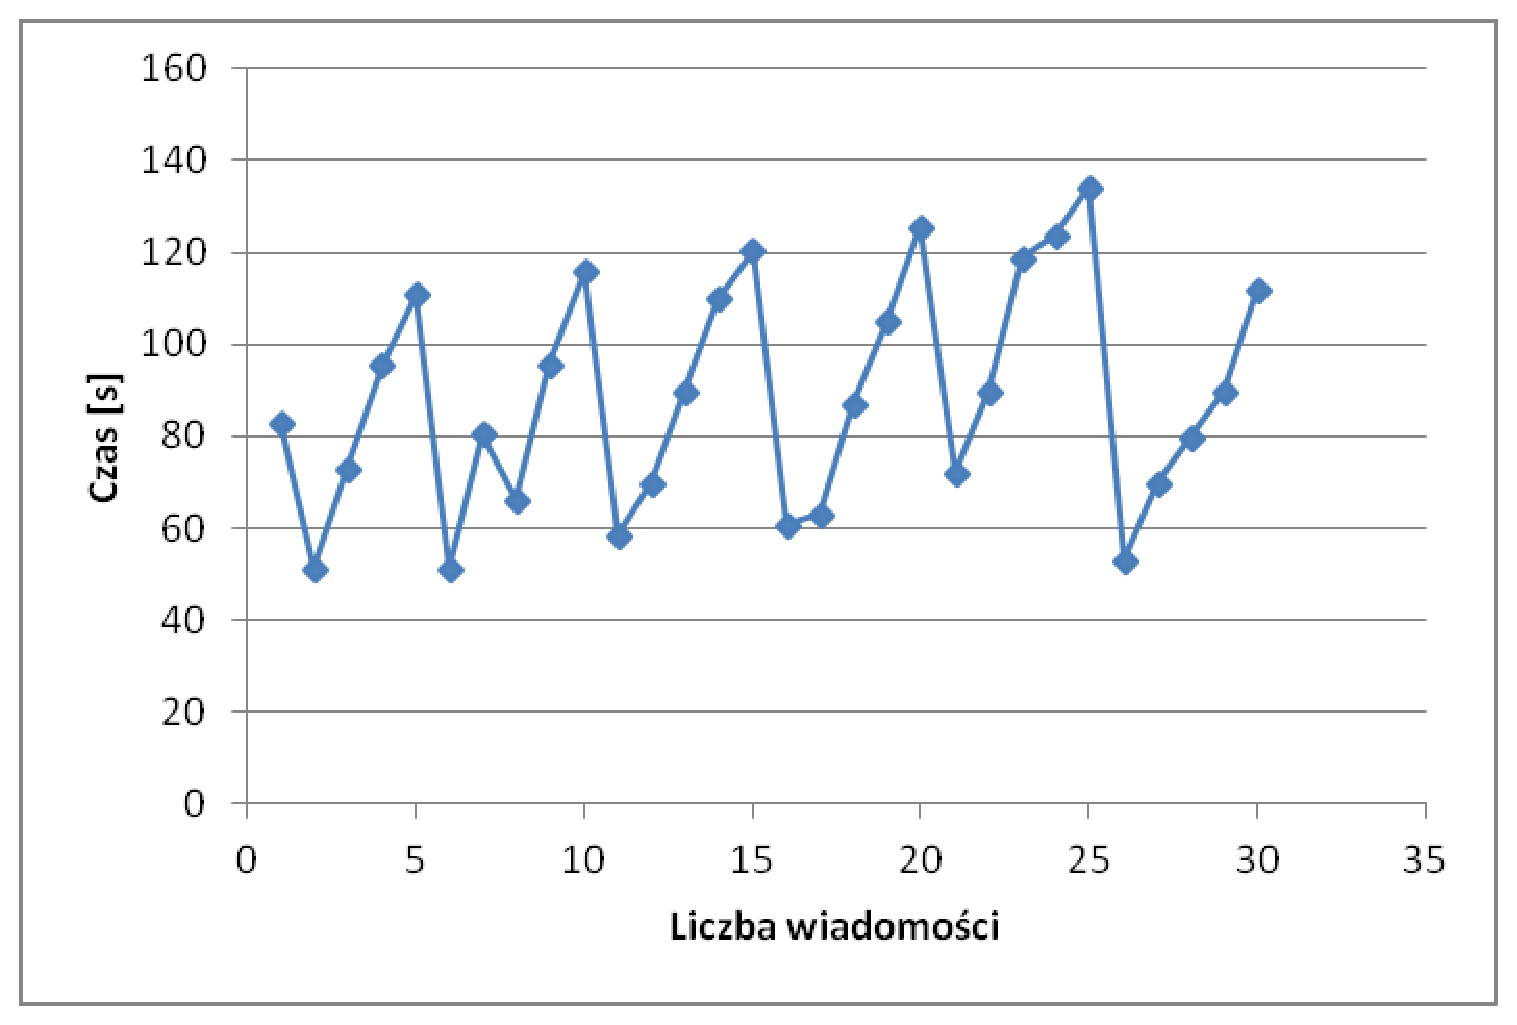
\includegraphics[width=0.8\linewidth]{img/kompaktowanie}
\par\end{centering}
\caption{Działanie algorytmu ZLT\label{fig:Dzia=000142anie-algorytmu-zmniejszaj=000105c}}
\end{figure}

Na osi poziomej znajduje się liczba wiadomości wysłanych przez nadawcę,
a~na pionowej — czas przesyłu. Zachowano domyślną liczbę wiadomości
umieszczanych w~torrencie kontrolnym — 5. W~drugim teście uczestniczyły
komputery K1 oraz komputer K2, który był nadawcą $U_{N}$ w~scenariuszu
2.

Minimalny czas przesyłu wiadomości zgadza się z~wynikiem uzyskanym
w~teście z~punktu \ref{sec:Wys=000142anie pojed wiad} — 50~sekund.
Wyniki na wykresie \ref{fig:Dzia=000142anie-algorytmu-zmniejszaj=000105c}
zostały uśrednione — w~testach brała udział różna liczba odbiorców.
Można zaobserwować spadek wydajności w~miarę zbliżania do momentu,
w~którym algorytm zmniejsza liczbę torrentów, po czym następuje wzrost
wydajności (zmniejszenie czasu przesyłu).

Należy dodać, że symulowana rozmowa nie odzwierciedla idealnie prawdziwej
sytuacji, w~której użytkownicy mogą nie odpowiedzieć na jakąś wiadomość,
lub odpowiedzieć poprzez wysłanie większej liczby wiadomości. W~tej
sytuacji algorytm ZLT może zmniejszać liczbę torrentów różnym użytkownikom
w~różnych momentach i~uzyskane czasy przesyłu wiadomości zostaną
uśrednione.

\section{Wpływ liczby wiadomości w~algorytmie ZLT}

\label{sec:wp=000142yw liczby wiad w zlt}

Kolejnym kryterium, które wzięto pod uwagę podczas testów była liczba
wiadomości, które algorytm ZLT umieszcza w~torrencie kontrolnym (liczba
ta będzie dalej nazywana \dcsstrong{zmienną X}). Algorytm okazuje
się niezbędny, ponieważ nadmierna liczba torrentów, które w~danym
momencie udostępnia klient, może spowodować jego błędne zatrzymanie. 

Im mniejsza wartość zmiennej X, tym częściej algorytm wykonuje zamianę
wielu torrentów na pojedynczy kontrolny. Skrajnym przypadkiem jest
umieszczanie każdej nowej wiadomości razem ze wszystkimi poprzednimi
w~nowym torrencie i~usunięcie poprzedniego torrenta. W~takiej sytuacji
liczba torrentów utrzymywanych przez każdego klienta byłaby równa
liczbie uczestników rozmowy. Jednakże, każda operacja zamiany wielu
torrentów na pojedynczy wymaga pewnego nakładu pracy, a~w~opisanym
przypadku koszt osiągnąłby wartość maksymalną. Dodatkowo, istnieje
narzut komunikacyjny spowodowany przesyłaniem tych samych wiadomości
ponownie w~połączonym torrencie. 

Im wyższa wartość zmiennej X, tym wyższa jest maksymalna liczba torrentów,
które klient będzie musiał utrzymywać z~powodu rzadziej następującej
zamiany. 

Wykresy \ref{fig:Liczba-wys=000142anych-wiadomo=00015Bci} i~\ref{fig:Liczba-wykona=000144-algorytmu}
przedstawiają zależności pewnych parametrów względem różnych wartości
zmiennej X. Oba wykresy bazują na 100 powtórzeniach wysłania wiadomości
(100 iteracji). Pierwszy wykres przedstawia, ile faktycznie wiadomości
wyśle klient — w~wynikach uwzględniono też powtórzone wiadomości,
które zostały wysłane wcześniej, a~znalazły się ponownie w~nowym
torrencie kontrolnym. Drugi wykres pokazuje: ile razy algorytm ZLT
stworzył nowy torrent (\glqq Wykonania'') oraz jaka jest maksymalna
liczba torrentów zaobserwowana w~trakcie 100 iteracji. 

\begin{figure}[tbph]
\begin{centering}
\includegraphics[width=0.8\linewidth]{\string"img/liczba wyslanych wiad od X\string".png}
\par\end{centering}
\caption{Liczba wysłanych wiadomości\label{fig:Liczba-wys=000142anych-wiadomo=00015Bci}}

\end{figure}

\begin{figure}[tbph]
\begin{centering}
\includegraphics[width=1\linewidth]{\string"img/wykonania i l torr od x\string".png}
\par\end{centering}
\caption{Liczba wykonań algorytmu i~maksymalna liczba torrentów\label{fig:Liczba-wykona=000144-algorytmu}}

\end{figure}

Z pierwszego wykresu wynika, że optymalna wartość zmiennej X wynosi
6 lub 8 — dla tych wartości zmiennej X liczba wysłanych wiadomości
jest najmniejsza. Zbadano również, że wraz ze wzrostem liczby iteracji
(więcej niż 100) optimum na pierwszym wykresie przesuwa się w~stronę
wyższej wartości X. Należy jednak pamiętać, że w~teście \ref{sec:Wp=000142yw alg}
(a~konkretnie próbie z~wyłączonym algorytmem ZLT) wykazano, iż maksymalna
liczba torrentów, jakie może obsłużyć aplikacja wynosi około 60-70.
Konieczne jest zatem minimalizowanie liczby jednocześnie uruchomionych
torrentów. 

Dodatkowo, każdy użytkownik, który aktywnie udziela się w~rozmowie,
powoduje wzrost liczby uruchomionych torrentów, które wszystkie klienty
w~konwersacji muszą obsłużyć. Przedstawione na wykresie wartości
dotyczą pojedynczego użytkownika. Gdyby, przykładowo, uczestników
było dwóch, maksymalna liczba torrentów podwaja się, w~przypadku
3 uczestników — potraja, itd. Można więc zauważyć, że przyjmując wartość
zmiennej X równą 10, możliwe jest przekroczenie 60 obsługiwanych torrentów
przy 4 uczestnikach rozmowy.

\section{Pobieranie listy wiadomości}

Ostatni test korzysta ze scenariusza 3. Jego celem jest pomiar czasu
potrzebnego na pobranie pełnej listy wiadomości przez użytkownika
dołączającego do trwającej rozmowy. Istotnymi kryteriami w~tym teście
są: liczba wiadomości do pobrania oraz zastosowana wartość zmiennej
X w~algorytmie ZLT. Wyniki przeprowadzonych doświadczeń nie odbiegają
od oczekiwań i~rezultatów poprzednich testów. 

Przede wszystkim, przy wyłączonym algorytmie ZLT konieczne byłoby
pobieranie każdej wiadomości z~osobna, jedna po drugiej, dlatego
całkowity czas pobrania wynosiłby $n\cdotp V$, gdzie $n$ oznacza
liczbę wiadomości do pobrania, a~$V$ — średni czas przesłania wiadomości
w~danym środowisku testowym. Włączenie algorytmu pozwala na znaczne
skrócenie całkowitego czasu. 

Czas ten można by jeszcze przyspieszyć, gdyby w~aplikacji zaimplementowany
został mechanizm przechowywania list ostatnich wartości info hash
(zamiast pojedynczych wartości) w~DHT oraz strukturze komunikatu
(wspomniany w~punkcie \ref{subsec:lista IH zamiast pojedynczych warto=00015Bci}).
W~takiej sytuacji część wiadomości mogłaby być pobierana równolegle.

Bez wspomnianego mechanizmu, czasy pobierania wiadomości w~sieci
laboratoryjnej pomiędzy komputerami K1 są dłuższe i~zostały przedstawione
na wykresie \ref{fig:Pobieranie-listy-wiadomo=00015Bci}. Liczba komputerów
biorących udział w~teście miała marginalne znaczenie. Każdy punkt
oznacza czas pobrania danej liczby wiadomości w~zależności od wartości
zmiennej X ustawionej w~algorytmie ZLT. 

\begin{figure}[tbph]
\includegraphics[width=1\linewidth]{\string"img/pobieranie listy\string".png}

\caption{Pobieranie listy wiadomości o~różnej długości\label{fig:Pobieranie-listy-wiadomo=00015Bci}}

\end{figure}

Można zaobserwować, że czas pobierania listy wiadomości jest tym dłuższy,
im więcej komunikatów zostało wysłanych od momentu utworzenia ostatniego
torrenta kontrolnego przez algorytm ZLT. Ponadto, dla wyższych wartości
zmiennej X istnieje możliwość większego oddalenia się od wspomnianego
torrenta. Przykładowo, dla zmiennej X równej 9 prawdopodobieństwo,
że konieczne będzie pobranie więcej niż 3 wiadomości zanim pobrany
zostanie torrent kontrolny wynosi 63\%, natomiast dla zmiennej X równej
3 — 0\%. Takie samo prawdopodobieństwo występuje na kolejnych poziomach
algorytmu. 

\section{Wpływ jednoczesnych konwersacji na wydajność}

W sieci domowej prędkości pobierania i~wysyłania danych są znacznie
mniejsze niż w~sieci laboratoryjnej. W~celu sprawdzenia, czy większa
liczba konwersacji wpływa na pogorszenie wydajności, uruchomiono 4
klienty aplikacji na komputerach K3 i~K4. Zaobserwowano porównywalne
pogorszenie wydajności aplikacji zarówno gdy klienty prowadzą wspólną
konwersację oraz gdy klienty prowadzą 2 konwersacje parami. Oznacza
to, że w~wolniejszych sieciach większy wpływ na wydajność ma liczba
włączonych klientów niż to, w~jaki sposób są one połączone (kto rozmawia
z~kim). 

W sieci laboratoryjnej test przeprowadzono na komputerach K1. Nie
zaobserwowano istotnej różnicy w~czasie przesłania wiadomości w~zależności
od tego, czy klienty prowadzą wspólną rozmowę, czy kilka osobnych. 

\section{Podsumowanie testów}

\label{sec:Podsumowanie test=0000F3w}

Z wyników testów oraz doświadczeń z~innymi aplikacjami wykorzystującymi
protokół BitTorrent można wywnioskować, że protokół znacznie lepiej
sprawdza się w~przypadku, gdy klient pobiera lub udostępnia niewielką
liczbę torrentów. Jednakże, pojedynczy torrent może i~powinien zawierać
możliwie dużo plików o~jak największym rozmiarze — wtedy jednorazowe,
dość kosztowne komunikacyjnie dołączenie do swarmu pozwala na pobranie
dużej ilości danych. Należy więc minimalizować liczbę jednocześnie
pobieranych torrentów, a~maksymalizować rozmiar lub liczbę plików
pobieranych w~ramach każdego z~nich. 

\chapter{Podsumowanie}

Podsumowując dotychczasowe rozważania i~wyniki testów należy przede
wszystkim zwrócić uwagę na fakt, że zakładany sposób funkcjonowania
systemu okazał się możliwy do osiągnięcia w~praktyce po drobnych
modyfikacjach. Komunikator umożliwia użytkownikom prowadzenie rozmów,
a~wiadomości są przekazywane wprost pomiędzy klientami, bez pośrednictwa
serwerów. Wprowadzono również algorytm ZLT (punkt \ref{subsec:Wysy=000142anie wiadomo=00015Bci})
oraz usuwanie torrentów starszych niż tydzień (punkt \ref{subsec:Udost=000119pnianie starych torr})
— funkcje mające na celu poprawę wydajności aplikacji. 

Niestety, testy wykazały, że czasy przesyłu wiadomości należałoby
w~dalszym ciągu znacząco poprawić. W~założeniach dowolnego komunikatora
dąży się do osiągnięcia czasu przesłania komunikatu bliskiego zero
(rozmowy w~czasie rzeczywistym). W~przypadku komunikatora będącego
przedmiotem niniejszej pracy, czas przesłania komunikatu wyniósł minimalnie
około 0,5~sekundy, ale notowano też przypadki wielokrotnie dłuższego
oczekiwania na dostarczenie. W~punkcie \ref{sec:Dalszy rozw=0000F3j}
zaproponowano rozwiązania mogące pozytywnie wpłynąć na wydajność systemu,
a~których z~różnych względów nie umieszczono w~projekcie. Zrezygnowano
z~wdrożenia szyfrowania wiadomości, a~powody szerzej opisano w~punkcie
\ref{sec:Bezpiecze=000144stwo, krypto, JS}.

Wykorzystanie protokołu BitTorrent umożliwiło skupienie się na implementacji
kluczowych funkcji systemu, logiki aplikacji. Skomunikowanie klientów
ze sobą było zadaniem protokołu. Dzięki temu rozwój aplikacji był
znacznie szybszy, w~porównaniu do sytuacji, w~której należałoby
zadbać również o~ten aspekt. Jednakże, w~ramach przyszłego rozwoju
aplikacji, należałoby wprowadzić pewne zmiany w~protokole — mowa
o~nich w~punktach \ref{subsec:zmiana zawarto=00015Bci bez zmiany IH}
oraz \ref{sec:Podsumowanie test=0000F3w}. 

Niniejsza praca magisterska może być traktowana jako źródło cennych
informacji związanych z~protokołem BitTorrent oraz implementacją
systemu rozproszonego komunikatora internetowego. W~szczególności,
może posłużyć do ponownego przemyślenia pewnych kwestii i~wdrożenia
kolejnej wersji komunikatora pozbawionego poznanych dotychczas wad.
Autor pracy ma nadzieję, że zalety architektury rozproszonej pozwolą
na ostateczne opracowanie komunikatora mogącego realnie konkurować
z~istniejącymi, scentralizowanymi produktami.

\selectlanguage{english}%

\appendix
\backmatter
\selectlanguage{polish}%
\begin{thebibliography}{10}
\bibitem{IM 1}Rebecca E. Grinter, Leysia Palen, \glqq Instant Messaging
in Teen Life'', University of Colorado, 2002, strony 21-22

\bibitem{IM 2}Jure Leskovec, Eric Horvitz, \glqq Planetary-Scale
Views on a~Large Instant-Messaging Network'', Microsoft Research,
2008, strony 1-2

\bibitem{IM 3}Anabel Quan-Haase, Alyson L. Young, \glqq Uses and
Gratifications of Social Media: A Comparison of Facebook and Instant
Messaging'', Bulletin of Science Technology \& Society, 2010, strony
350-352

\bibitem{messenger uzytkownicy}https://messenger.fb.com/?ref=platform
(dostęp 11.07.2017)

\bibitem{messenger u=00017Cytkownicy 2}https://techcrunch.com/2017/04/12/messenger/
(dostęp 11.07.2017)

\bibitem{miliardy}https://www.theverge.com/2016/4/12/11415198/facebook-messenger-whatsapp-number-messages-vs-sms-f8-2016
(dostęp 25.07.2017)

\bibitem{p2p 1}Ralf Steinmetz, \glqq Peer-to-Peer Systems and Applications'',
Springer-Verlag Berlin Heidelberg, 2005, strony 9-16

\bibitem{p2p 2}Quang H. Vu, \glqq Peer-to-Peer Computing: Principles
and Applications'', Springer, 2010, strony 1-10

\bibitem{fb-personalizowane reklamy}https://www.facebook.com/help/568137493302217
(dostęp 09.06.2017)

\bibitem{messenger}https://pl-pl.messenger.com/ (dostęp 09.06.2017)

\bibitem{messenger-encryption}https://www.facebook.com/help/messenger-app/811527538946901?helpref=uf\_permalink
(dostęp 13.06.2017)

\bibitem{bleep}http://www.bleep.pm/ (dostęp 09.06.2017)

\bibitem{bleep how it works}http://blog.bittorrent.com/2014/07/30/building-an-engine-for-decentralized-communications/
(dostęp 11.07.2017)

\bibitem{signal}https://whispersystems.org/ (dostęp 09.06.2017)

\bibitem{signal artyku=000142}Katriel Cohn-Gordon, Cas Cremers, Luke
Garratt i~inni, \glqq A Formal Security Analysis of the Signal Messaging
Protocol'', University of Oxford, 2016, (raport techniczny), https://eprint.iacr.org/2016/1013.pdf
(dostęp 11.07.2017) 

\bibitem{wire}https://wire.com/en/ (dostęp 11.07.2017)

\bibitem{wire privacy rep}\glqq Wire Privacy Whitepaper'', Wire
Swiss GmbH, 2017, (raport techniczny), https://wire.com/resource/Wire\%20Privacy\%20Whitepaper/download/
(dostęp 11.07.2017)

\bibitem{wire security rep}\glqq Wire Security Whitepaper'', Wire
Swiss GmbH, 2017, (raport techniczny), https://wire.com/resource/Wire\%20Security\%20Whitepaper/download/
(dostęp 11.07.2017)

\bibitem{telegram}https://telegram.org/ (dostęp 11.07.2017)

\bibitem{telegram protok=0000F3=000142}https://core.telegram.org/mtproto
(dostęp 11.07.2017)

\bibitem{allo}https://allo.google.com/ (dostęp 11.07.2017)

\bibitem{whatsapp}https://www.whatsapp.com/ (dostęp 27.06.2017)

\bibitem{whatsapp whitepaper}\glqq WhatsApp Encryption Overview,
Technical white paper'', WhatsApp, 2017, (raport techniczny), https://www.whatsapp.com/security/WhatsApp-Security-Whitepaper.pdf
(dostęp 11.07.2017)

\bibitem{darkwire}https://darkwire.io/ (dostęp 09.06.2017)

\bibitem{darkwire git}https://github.com/seripap/darkwire.io (dostęp
11.07.2017)

\bibitem{friends}http://moose-team.github.io/friends/ (dostęp 09.06.2017)

\bibitem{merkle}Georg Becker, \glqq Merkle Signature Schemes, Merkle
Trees and Their Cryptanalysis\char`\"{}. Ruhr-Universität Bochum,
2008, http://www.emsec.rub.de/media/crypto/attachments/files/2011/04/becker\_1.pdf
(dostęp 09.06.2017)

\bibitem{tox}https://tox.chat/ (dostęp 09.06.2017)

\bibitem{tox faq}https://tox.chat/faq.html\#techfaq (dostęp 11.07.2017)

\bibitem{zeronet}https://zeronet.readthedocs.io/en/latest/using\_zeronet/sample\_sites/
(dostęp 09.06.2017)

\bibitem{bitmessage-main}https://bitmessage.org/wiki/Main\_Page (dostęp
09.06.2017)

\bibitem{bitmessage-pdf}Jonathan Warren, \glqq Bitmessage: A Peer-to-Peer
Message Authentication and Delivery System'', 2012, (raport techniczny),
https://bitmessage.org/bitmessage.pdf (dostęp 09.06.2017)

\bibitem{tanenbaum causal order}Tanenbaum A. S., \glqq Distributed
Systems Principles and Paradigms'', Prentice Hall, 2007, strony 244-251

\bibitem{email-liczba}\glqq Email Statistics Report, 2017-2021'',
THE RADICATI GROUP, INC., http://www.radicati.com/wp/wp-content/uploads/2017/01/Email-Statistics-Report-2017-2021-Executive-Summary.pdf
(dostęp 12.07.2017)

\bibitem{bittorrent}http://www.bittorrent.org/ (dostęp 09.06.2017)

\bibitem{bittorrent pdf}Bram Cohen, \glqq Incentives Build Robustness
in BitTorrent'', 2003, 5 stron, http://www.bittorrent.org/bittorrentecon.pdf
(dostęp 14.07.2017)

\bibitem{magnet link}http://bittorrent.org/beps/bep\_0009.html (dostęp
09.06.2017)

\bibitem{magnet uri scheme}http://magnet-uri.sourceforge.net/ (dostęp
09.06.2017)

\bibitem{webtorrent}https://webtorrent.io/ (dostęp 09.06.2017)

\bibitem{webtorrent github}https://github.com/webtorrent/webtorrent
(dostęp 09.06.2017)

\bibitem{vuze wiki}https://wiki.vuze.com/w/WebTorrent (dostęp 14.07.2017)

\bibitem{webrtc}https://webrtc.org/ (dostęp 27.06.2017)

\bibitem{python-eve}http://python-eve.org/ (dostęp 09.06.2017)

\bibitem{bep39-bt}http://www.bittorrent.org/beps/bep\_0039.html (dostęp
28.06.2017)

\bibitem{bep46-bt}http://www.bittorrent.org/beps/bep\_0046.html (dostęp
09.06.2017)

\bibitem{bep46-wt}https://github.com/webtorrent/webtorrent/issues/886
(dostęp 09.06.2017)

\bibitem{kademlia-dht}https://github.com/jeanlauliac/kademlia-dht
(dostęp 09.06.2017)

\bibitem{kadtools}https://github.com/kadtools/kad (dostęp 09.06.2017)

\bibitem{web cryptography api}https://developer.mozilla.org/en-US/docs/Web/API/Window/crypto
(dostęp 09.06.2017)

\bibitem{darkwire szyfrowanie how it works}https://github.com/seripap/darkwire.io\#how-it-works
(dostęp 09.06.2017)

\bibitem{signal double ratchet}Trevor Perrin, Moxie Marlinspike,
\glqq The Double Ratchet Algorithm'', 2016, (raport techniczny),
https://whispersystems.org/docs/specifications/doubleratchet/doubleratchet.pdf
(dostęp 13.06.2017)

\bibitem{bleep forward secrecy}http://engineering.bittorrent.com/2014/12/11/authentication-and-forward-secrecy-in-bleep/
(dostęp 14.06.2017)

\bibitem{bleep forward secrecy offline}http://engineering.bittorrent.com/2015/08/06/forward-secrecy-for-offline-messages-in-bleep/
(dostęp 14.06.2017)

\bibitem{webCrypto API w3}https://www.w3.org/TR/WebCryptoAPI/ (dostęp
09.06.2017)

\bibitem{webCrypto-experimental }https://developer.mozilla.org/en-US/docs/Web/API/Web\_Crypto\_API
(dostęp 09.06.2017)

\bibitem{wireshark}https://www.wireshark.org/ (dostęp 11.07.2017)

\bibitem{angularjs}https://angularjs.org/ (dostęp 11.07.2017)

\bibitem{grunt}https://gruntjs.com/ (dostęp 11.07.2017)

\bibitem{bower}https://bower.io/ (dostęp 11.07.2017)

\bibitem{yeoman}http://yeoman.io/ (dostęp 11.07.2017)

\bibitem{lodash}https://lodash.com/ (dostęp 11.07.2017)

\bibitem{node}https://nodejs.org/en/ (dostęp 11.07.2017)

\bibitem{express}https://expressjs.com/ (dostęp 11.07.2017)

\bibitem{npm}https://www.npmjs.com/ (dostęp 11.07.2017)

\bibitem{mongo}https://www.mongodb.com/ (dostęp 11.07.2017)

\bibitem{mlab}https://mlab.com/ (dostęp 11.07.2017)

\bibitem{protractor}http://www.protractortest.org/ (dostęp 11.07.2017)

\bibitem{heroku}https://www.heroku.com/ (dostęp 11.07.2017)
\end{thebibliography}

\end{document}
